\documentclass{../lab}
\usepackage[section]{placeins}

\labacronym{SHE}
\labtitle{Hall Effect in Semiconductor}

%\newcommand{\VanDerPauwTheorem}{http://experimentationlab.berkeley.edu/node/105}
%\newcommand{\CryogenicLiquids}{http://experimentationlab.berkeley.edu/sites/default/files/images/77cryogenic.pdf}
%\newcommand{\E.HallerArticle}{http://physics111.lib.berkeley.edu/Physics111/Reprints/SHE/24-Haller.pdf}
%\newcommand{\Solids}{http://physics111.lib.berkeley.edu/Physics111/Reprints/SHE/Halliday_Resnick/Ch.\%2046\%20Conduction\%20of\%20electricity\%20in\%20solids.pdf}

\begin{document}

\maketitle

\tableofcontents

\section{Hall Effect in a Semiconductor Description (SHE)}

\begin{enumerate}
    \item \textbf{Note that there is NO eating or drinking in the 111-Lab anywhere, except in rooms 282 \& 286 LeConte on the bench with the BLUE stripe around it.} Thank You the Staff.

\end{enumerate}

In general the Hall effect refers to the fact that a voltage can develop in a direction transverse to the current flow in a system of charged particles in a magnetic field, owing to the \href{http://experimentationlab.berkeley.edu/sites/default/files/Lorentz\%20force.pdf}{\textbf{Lorentz force}} $q(\mathbf{v} \times \mathbf{B})$.

The electrical resistance of conductors and non-conductors is relatively easy to describe conceptually and mathematically, and experiments illustrating these properties are easy to do. We are all familiar with Ohm's law, and with using dielectrics as insulators. The temperature dependence is nothing unusual. Semiconductors fall in between these two extremes, and their properties require some knowledge of condensed matter physics. The Hall effect illustrates the Lorentz force $\mathbf{v} \times \mathbf{B}$. In this experiment you will measure the resistivity and the Hall coefficient as functions of the temperature, for an Al-doped germanium crystal. You will then determine the concentration of the free carrier. When a current is passed through a sample in the x-direction the Lorentz force acting on the electric charges moving in a magnetic field \textbf{B} (in Z) displaces some carriers in the y-direction. This causes an internal electric field $\mathbf{E}_{H}$ which cancels the Lorentz force in the equilibrium case. You will use the Van der Pauw method of measuring a sample of arbitrary shape using the computer running LabView to acquire these data. The temperature range of this experiment is 300K to 77K to 400K.

\begin{enumerate}
    \item Pre-requisites: None

    \item Days Allotted for the Experiment: 5
\end{enumerate}

\noindent\textbf{All pages in this lab}

\begin{enumerate}
    \item \textbf{Hall Effect in Semiconductor}

    \item \href{http://experimentationlab.berkeley.edu/node/105}{\textbf{Van Der Pauw Theorem}}
    
    \item \href{http://experimentationlab.berkeley.edu/node/106}{\textbf{Instrument Manuals}}
\end{enumerate}

This lab will be graded 30\% on theory, 20\% on technique, and 50\% on analysis. For more information, see the \href{http://experimentationlab.berkeley.edu/syllabus}{\textbf{Advanced Lab Syllabus.}}

Comments: \Feedback

\textbf{Acknowledgment and Disclaimer} ``This material is based upon work supported by the National Science Foundation under Grant No. 9850553 ''Any opinions, findings and conclusions or recommendations expressed in this material are those of the author(s) and do not necessarily reflect the views of the National Science Foundation (NSF)."

This manual is intended to provide a general guidance for the lab. It is not designed to explain all the physics necessary for understanding this experiment, nor is it a "cook-book" telling you exactly which buttons to press, etc. It is up to the student to become familiar with the necessary material in the reprints, and to figure out the exact procedure necessary for completing the assignments in the lab. Talk with an instructor often, but not until you have given the physics and procedures some thought first. We are here to instruct and help, but not to do the thinking for you.

\section{Hall Effect in a Semiconductor Pictures (SHE)}

\noindent
\begin{figure}[H]
\captionsetup{justification=centering}
\minipage[t]{0.307\linewidth}
  \href{http://experimentationlab.berkeley.edu/sites/default/files/images/SHE_3541_Crop.jpg}{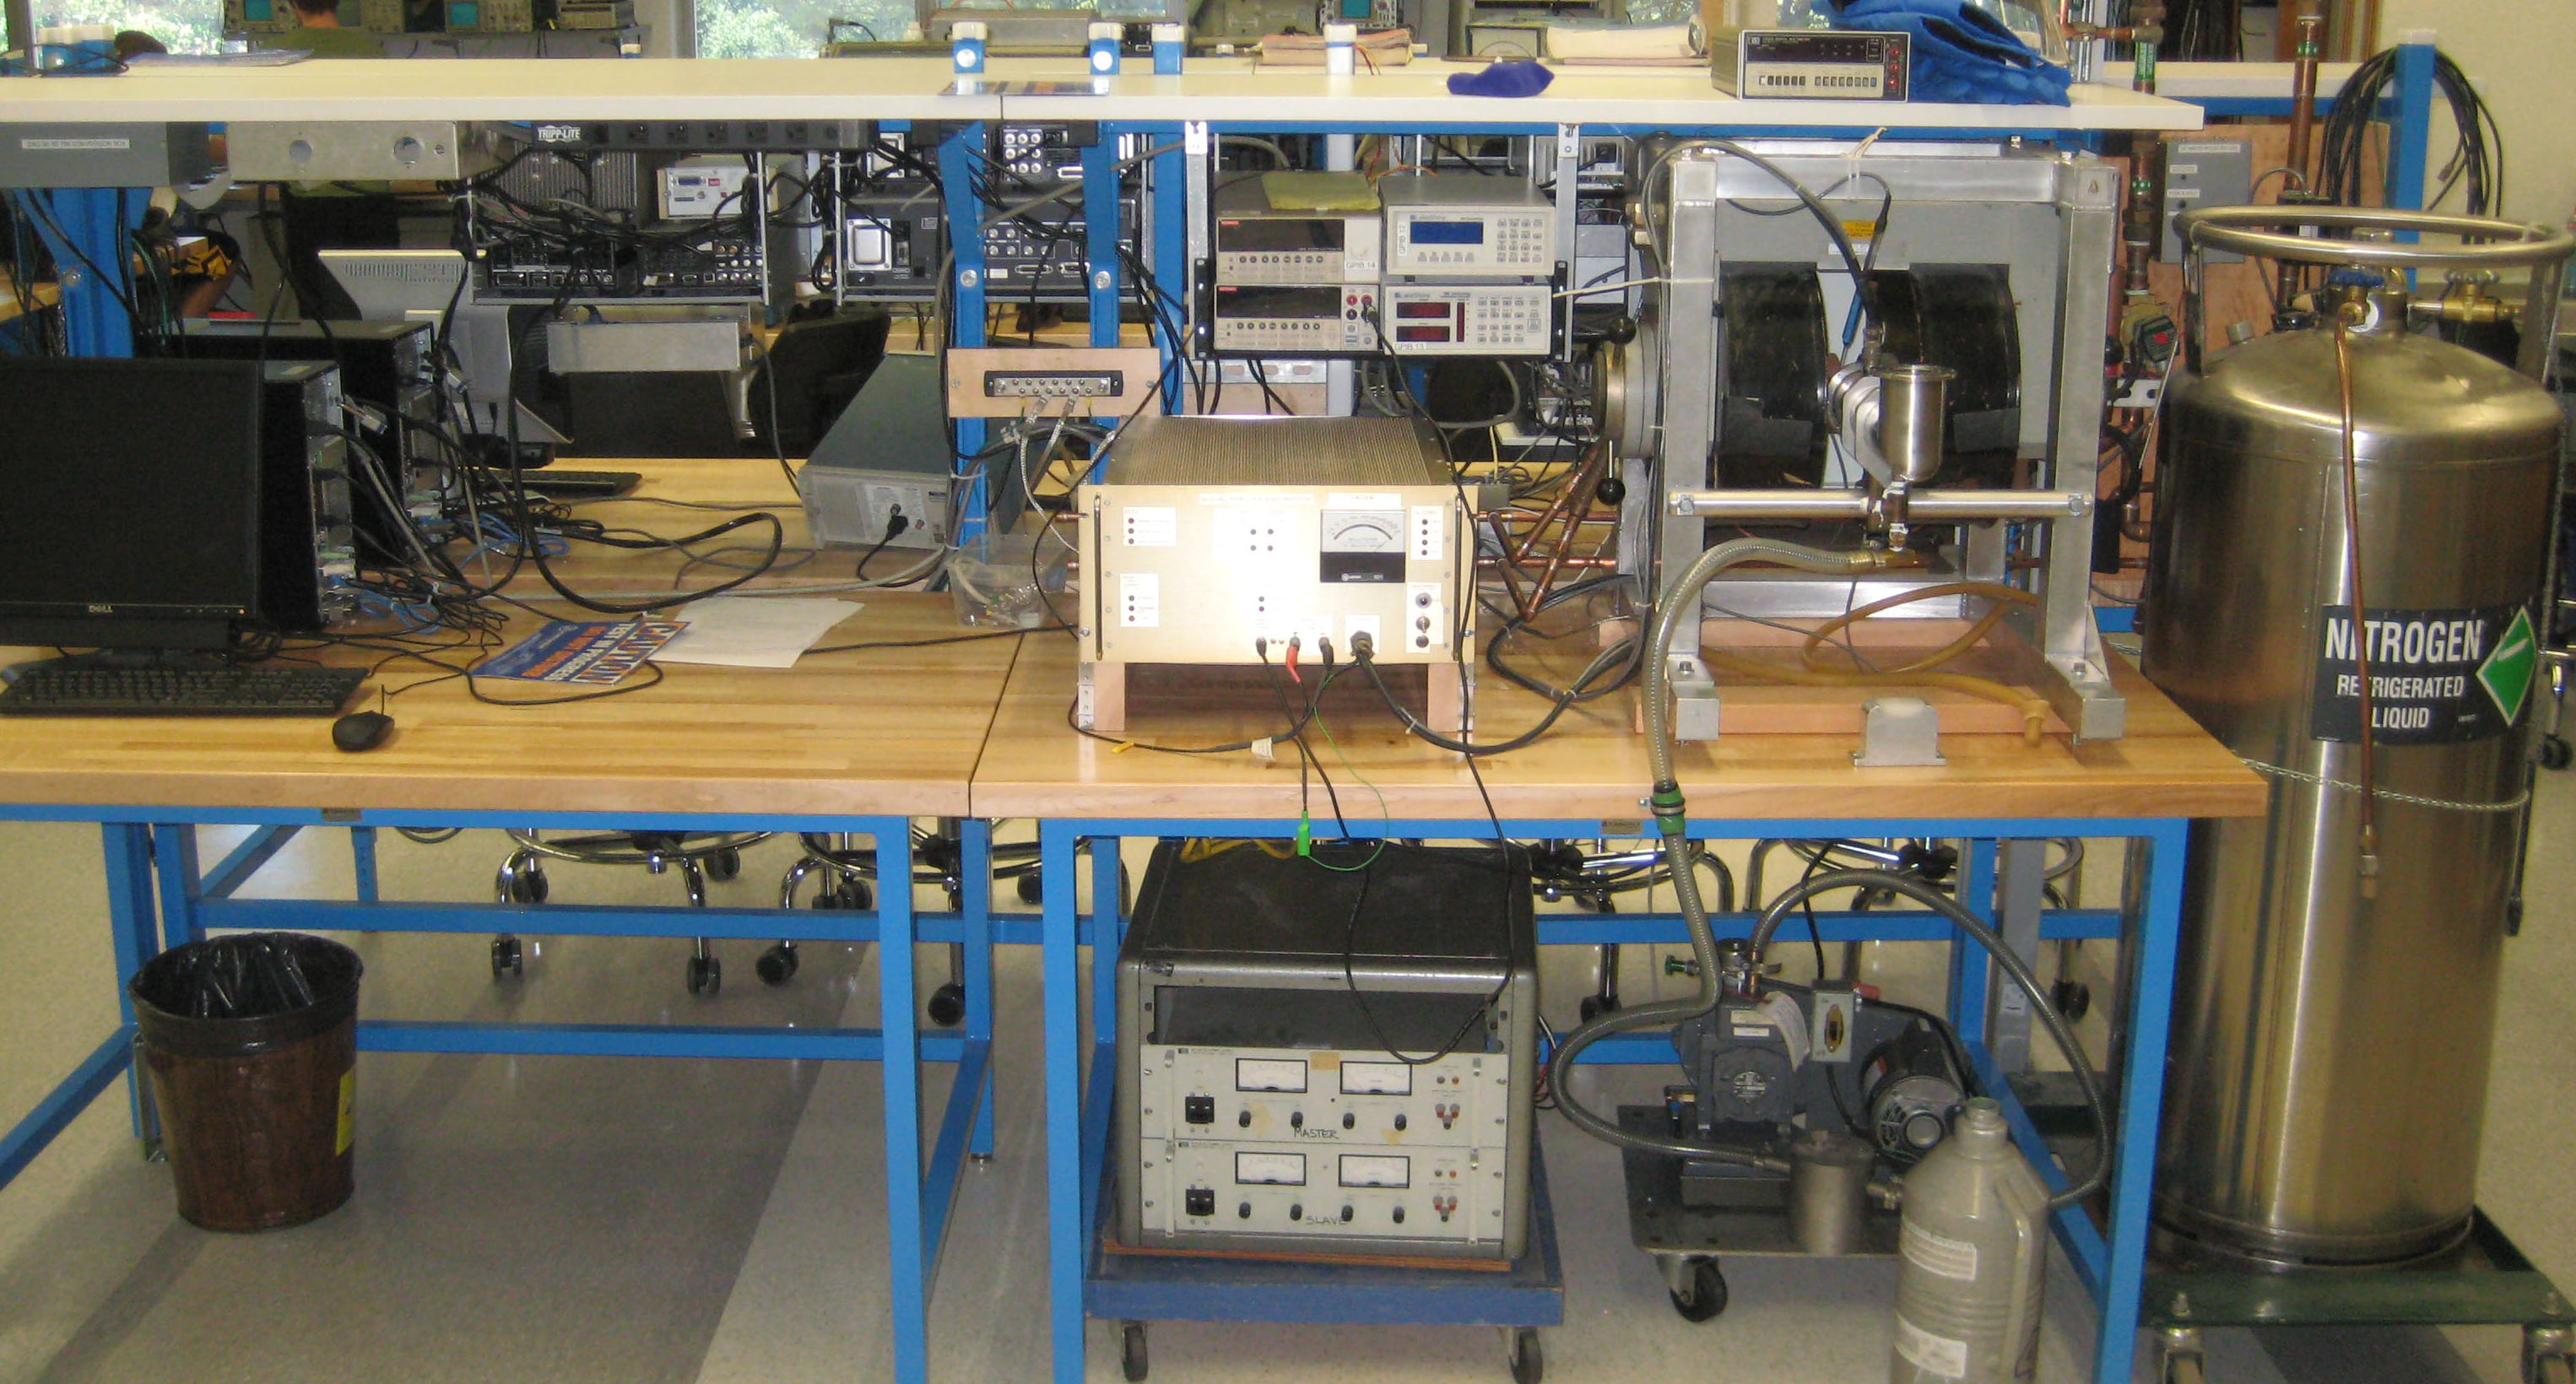
\includegraphics[width=\linewidth,keepaspectratio]{images/SHE_3541_Crop.jpg}}
  \caption{Hall Effect in a Semiconductor Experiment \\ \href{http://experimentationlab.berkeley.edu/sites/default/files/images/SHE_3541_Crop.jpg}{Click here to see larger picture}}
  \label{fig:SHE_3541_Crop.jpg}
\endminipage\hfill
\minipage[t]{0.166\linewidth}
  \href{http://experimentationlab.berkeley.edu/sites/default/files/images/SHE_Electronics_3546_Crop.jpg}{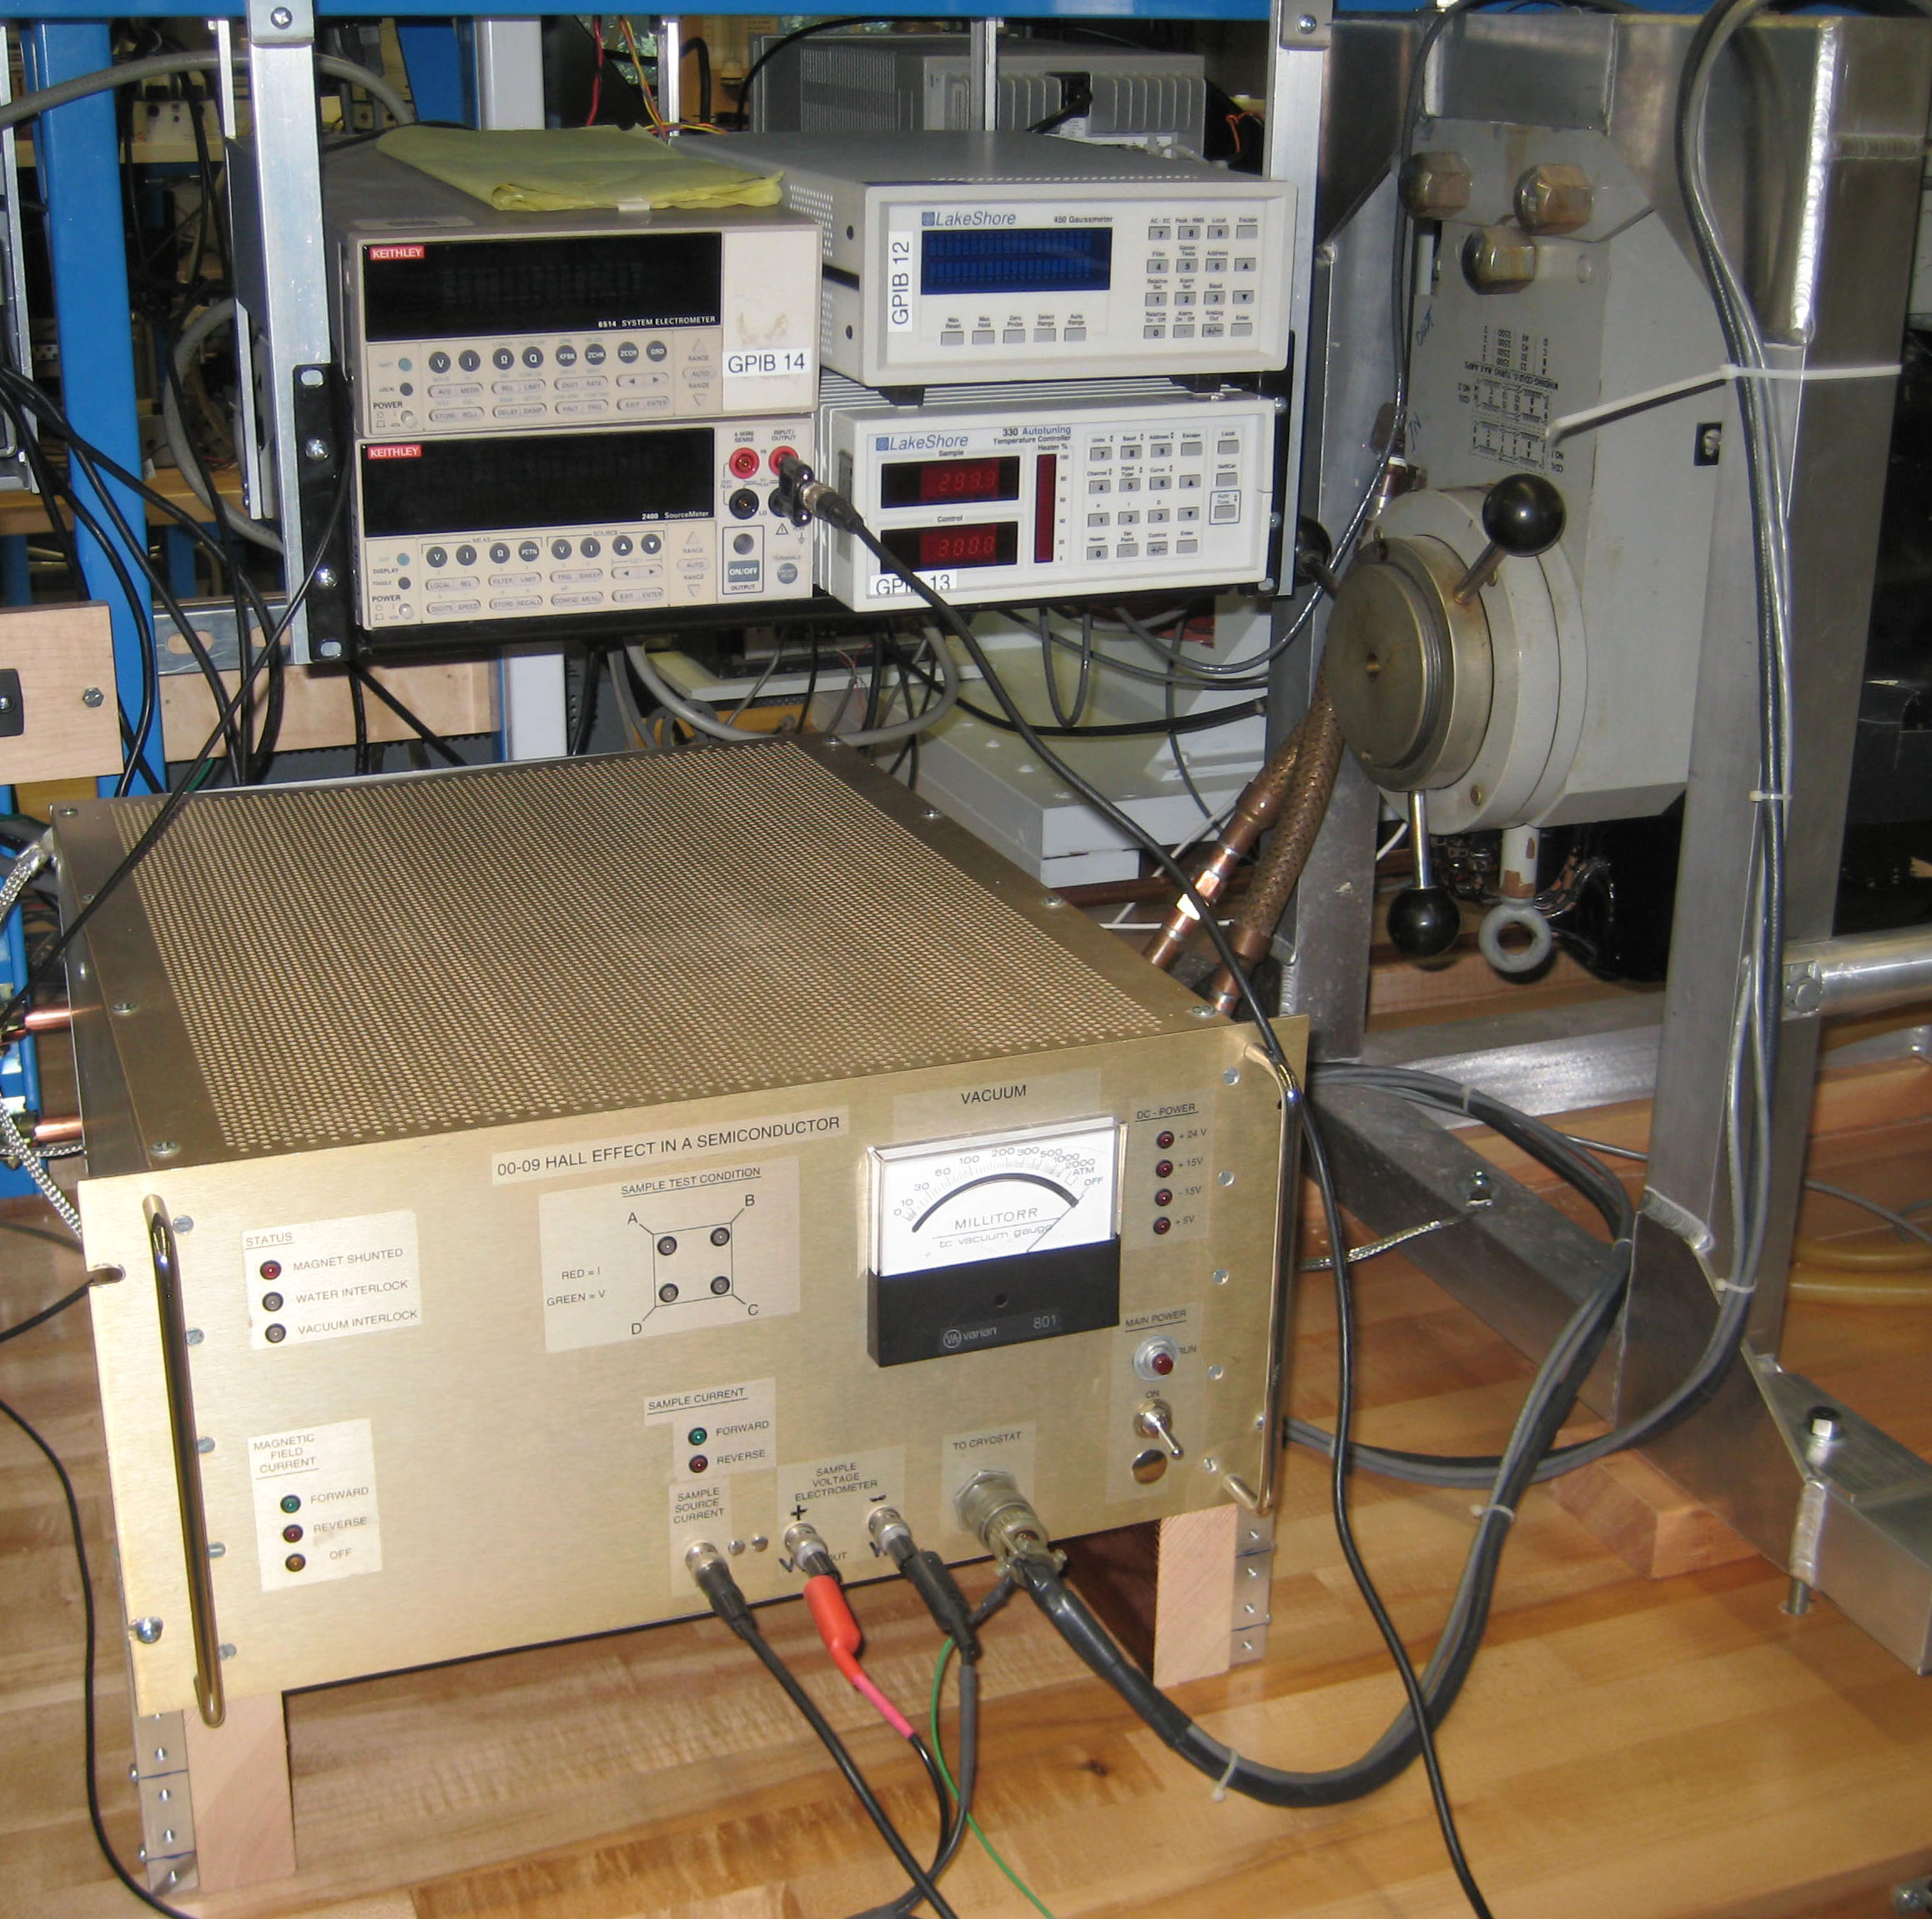
\includegraphics[width=\linewidth,keepaspectratio]{images/SHE_Electronics_3546_Crop.jpg}}
  \caption{Experiment Electronics \\
  \href{http://experimentationlab.berkeley.edu/sites/default/files/images/SHE_Electronics_3546_Crop.jpg}{Click here to see larger picture}}
  \label{fig:SHE_Electronics_3546_Crop.jpg}
\endminipage\hfill
\minipage[t]{0.288\linewidth}
  \href{http://experimentationlab.berkeley.edu/sites/default/files/images/SHE_Mag_Pwr_Crop_3547.jpg}{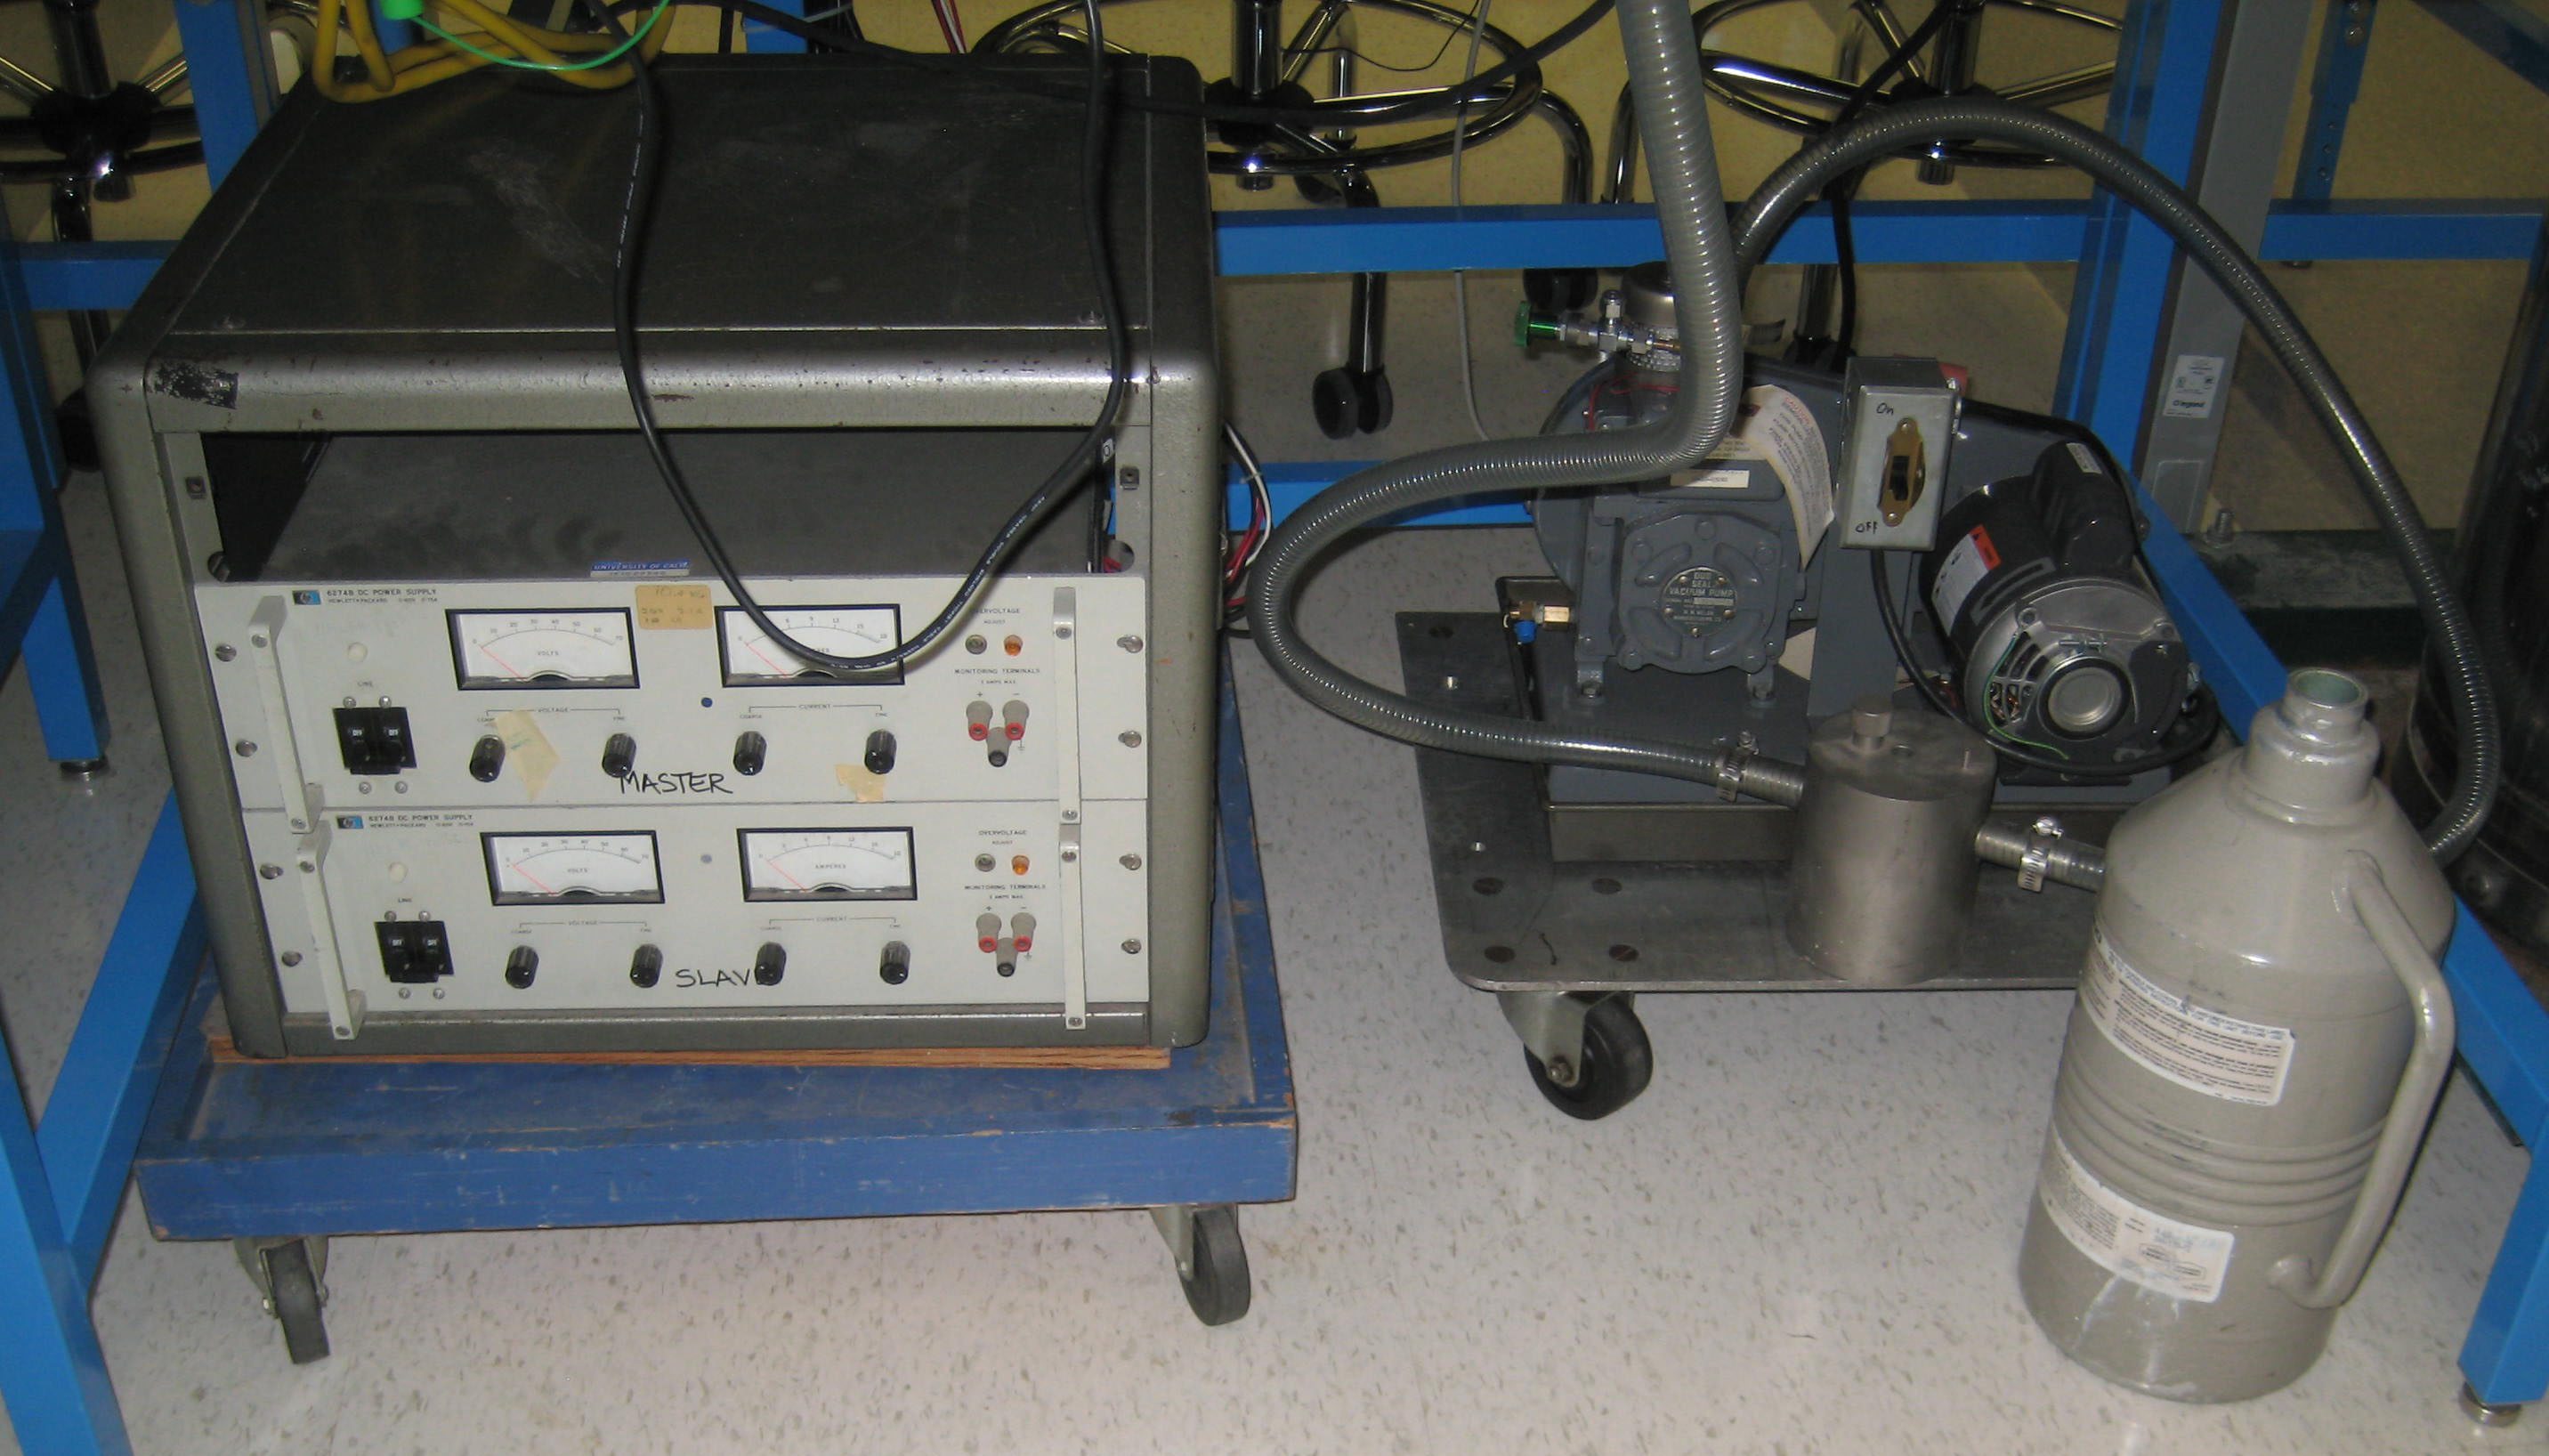
\includegraphics[width=\linewidth,keepaspectratio]{images/SHE_Mag_Pwr_Crop_3547.jpg}}
  \caption{Magnet Power Supply \& Vacuum Pump with Transfer LN-2 Dewar \\ \href{http://experimentationlab.berkeley.edu/sites/default/files/images/SHE_Mag_Pwr_Crop_3547.jpg}{Click here to see larger picture}}\label{fig:SHE_Mag_Pwr_Crop_3547.jpg}
\endminipage\hfill
\minipage[t]{0.219\linewidth}
  \href{http://experimentationlab.berkeley.edu/sites/default/files/images/Chamber_Front_3304.jpg}{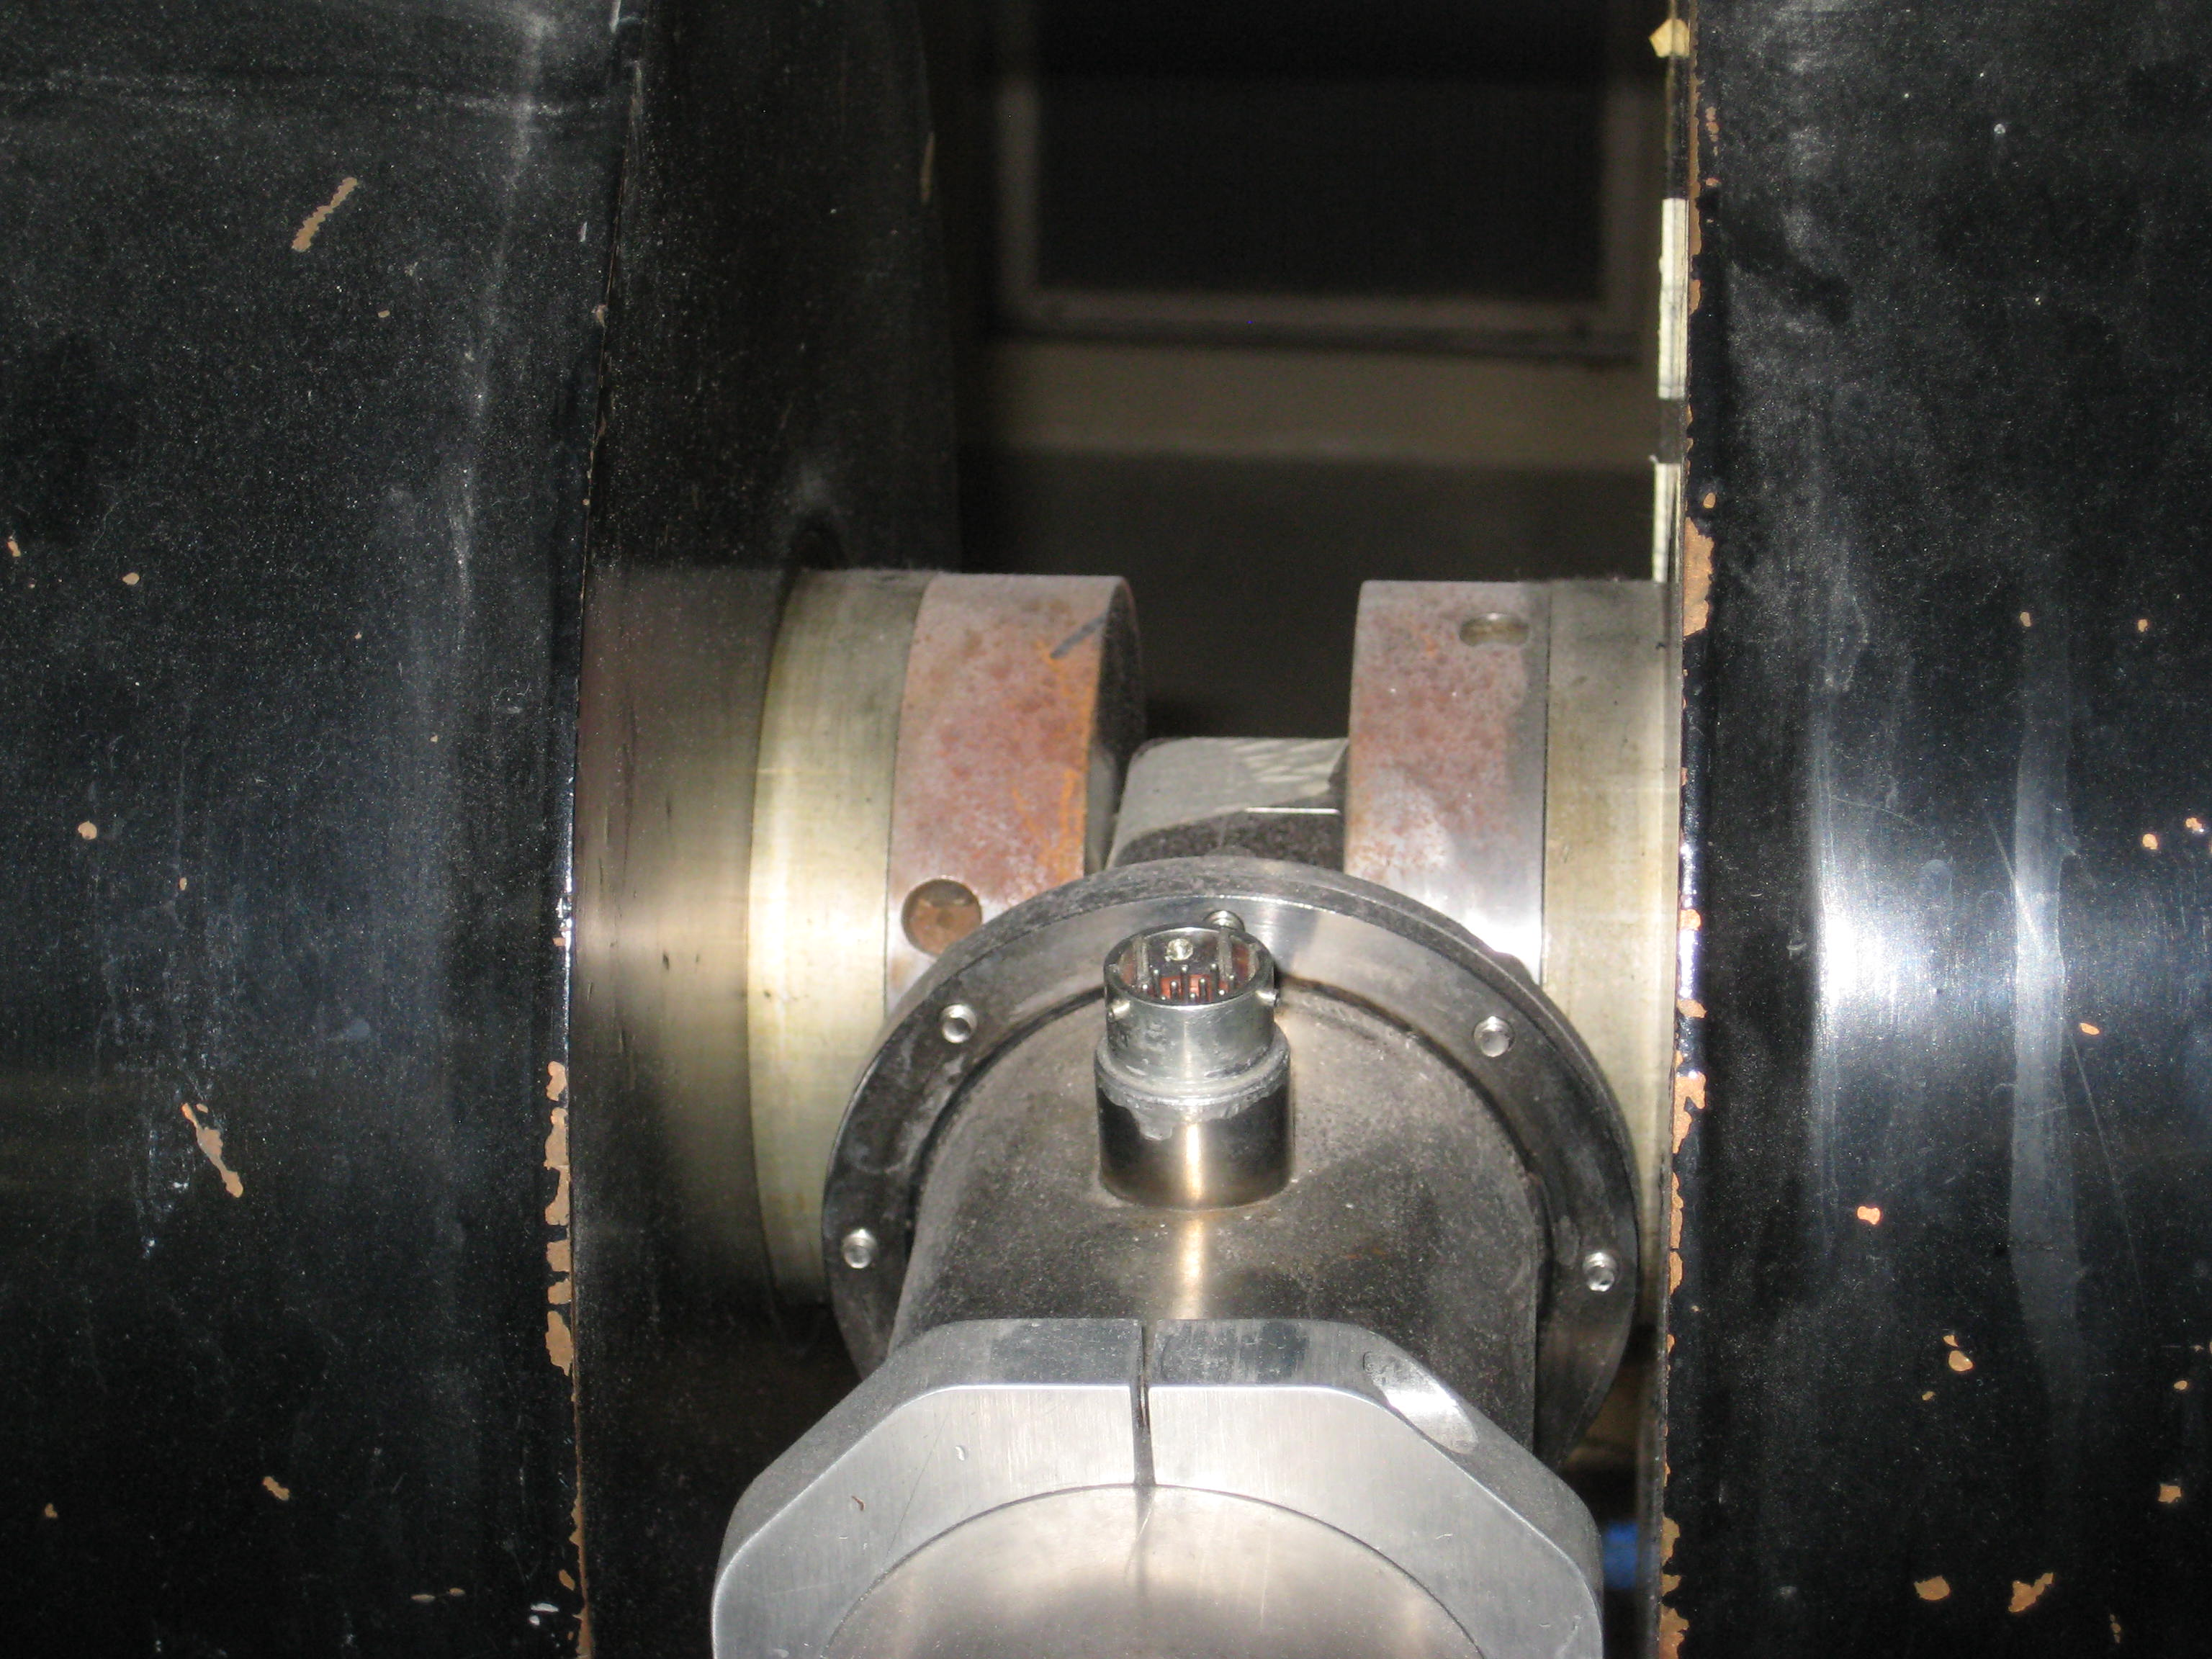
\includegraphics[width=\linewidth,keepaspectratio]{images/Chamber_Front_3304.jpg}}
  \caption{Chamber Front in Magnet \\ \href{http://experimentationlab.berkeley.edu/sites/default/files/images/Chamber_Front_3304.jpg}{Click here to see larger picture}}\label{fig:Chamber_Front_3304.jpg}
\endminipage
\end{figure}

\begin{figure}[H]
\captionsetup{justification=centering}
\minipage[t]{0.33\linewidth}
  \href{http://experimentationlab.berkeley.edu/sites/default/files/images/SHEimageFrontPanel.jpg}{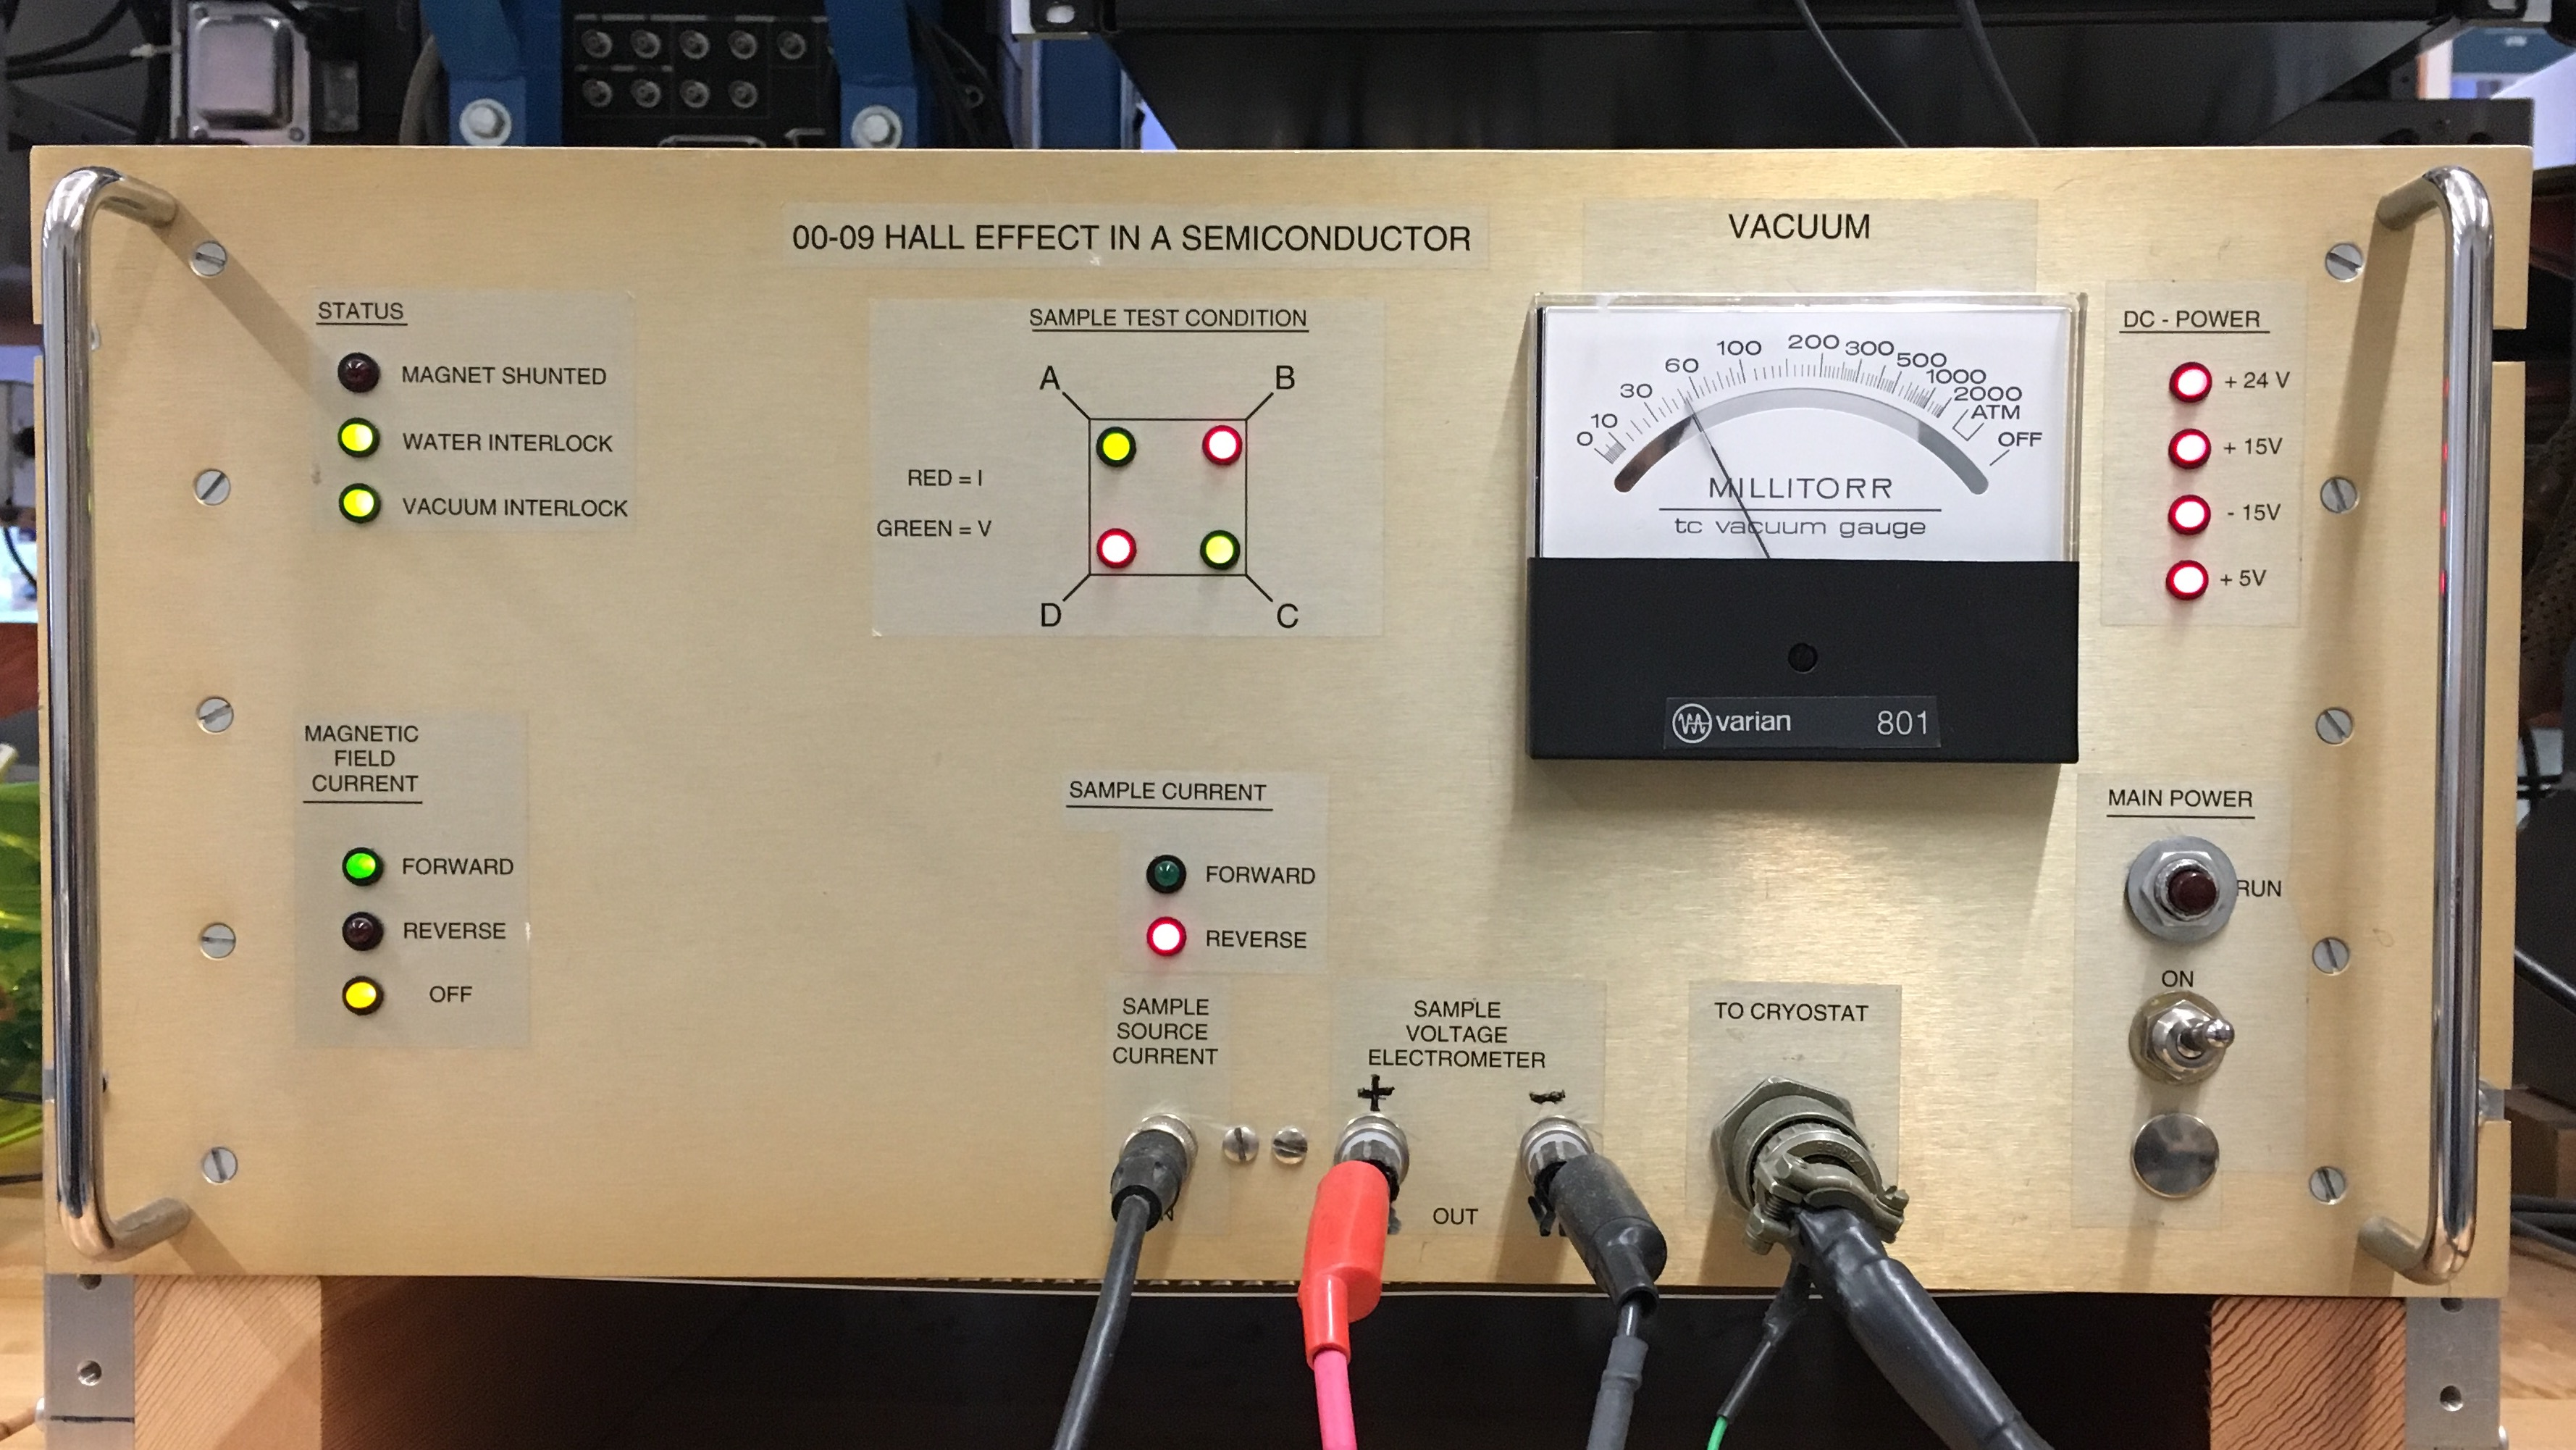
\includegraphics[width=\linewidth,keepaspectratio]{images/SHEimageFrontPanel.jpg}}
  \caption{The Gold Box which is operating\\ \href{http://experimentationlab.berkeley.edu/sites/default/files/images/SHEimageFrontPanel.jpg}{Click here to see larger picture}}
  \label{fig:GoldBox.jpg}
\endminipage\hfill
\minipage[t]{0.33\linewidth}
  \href{http://experimentationlab.berkeley.edu/sites/default/files/images/SHEimageGaussProbe.jpg}{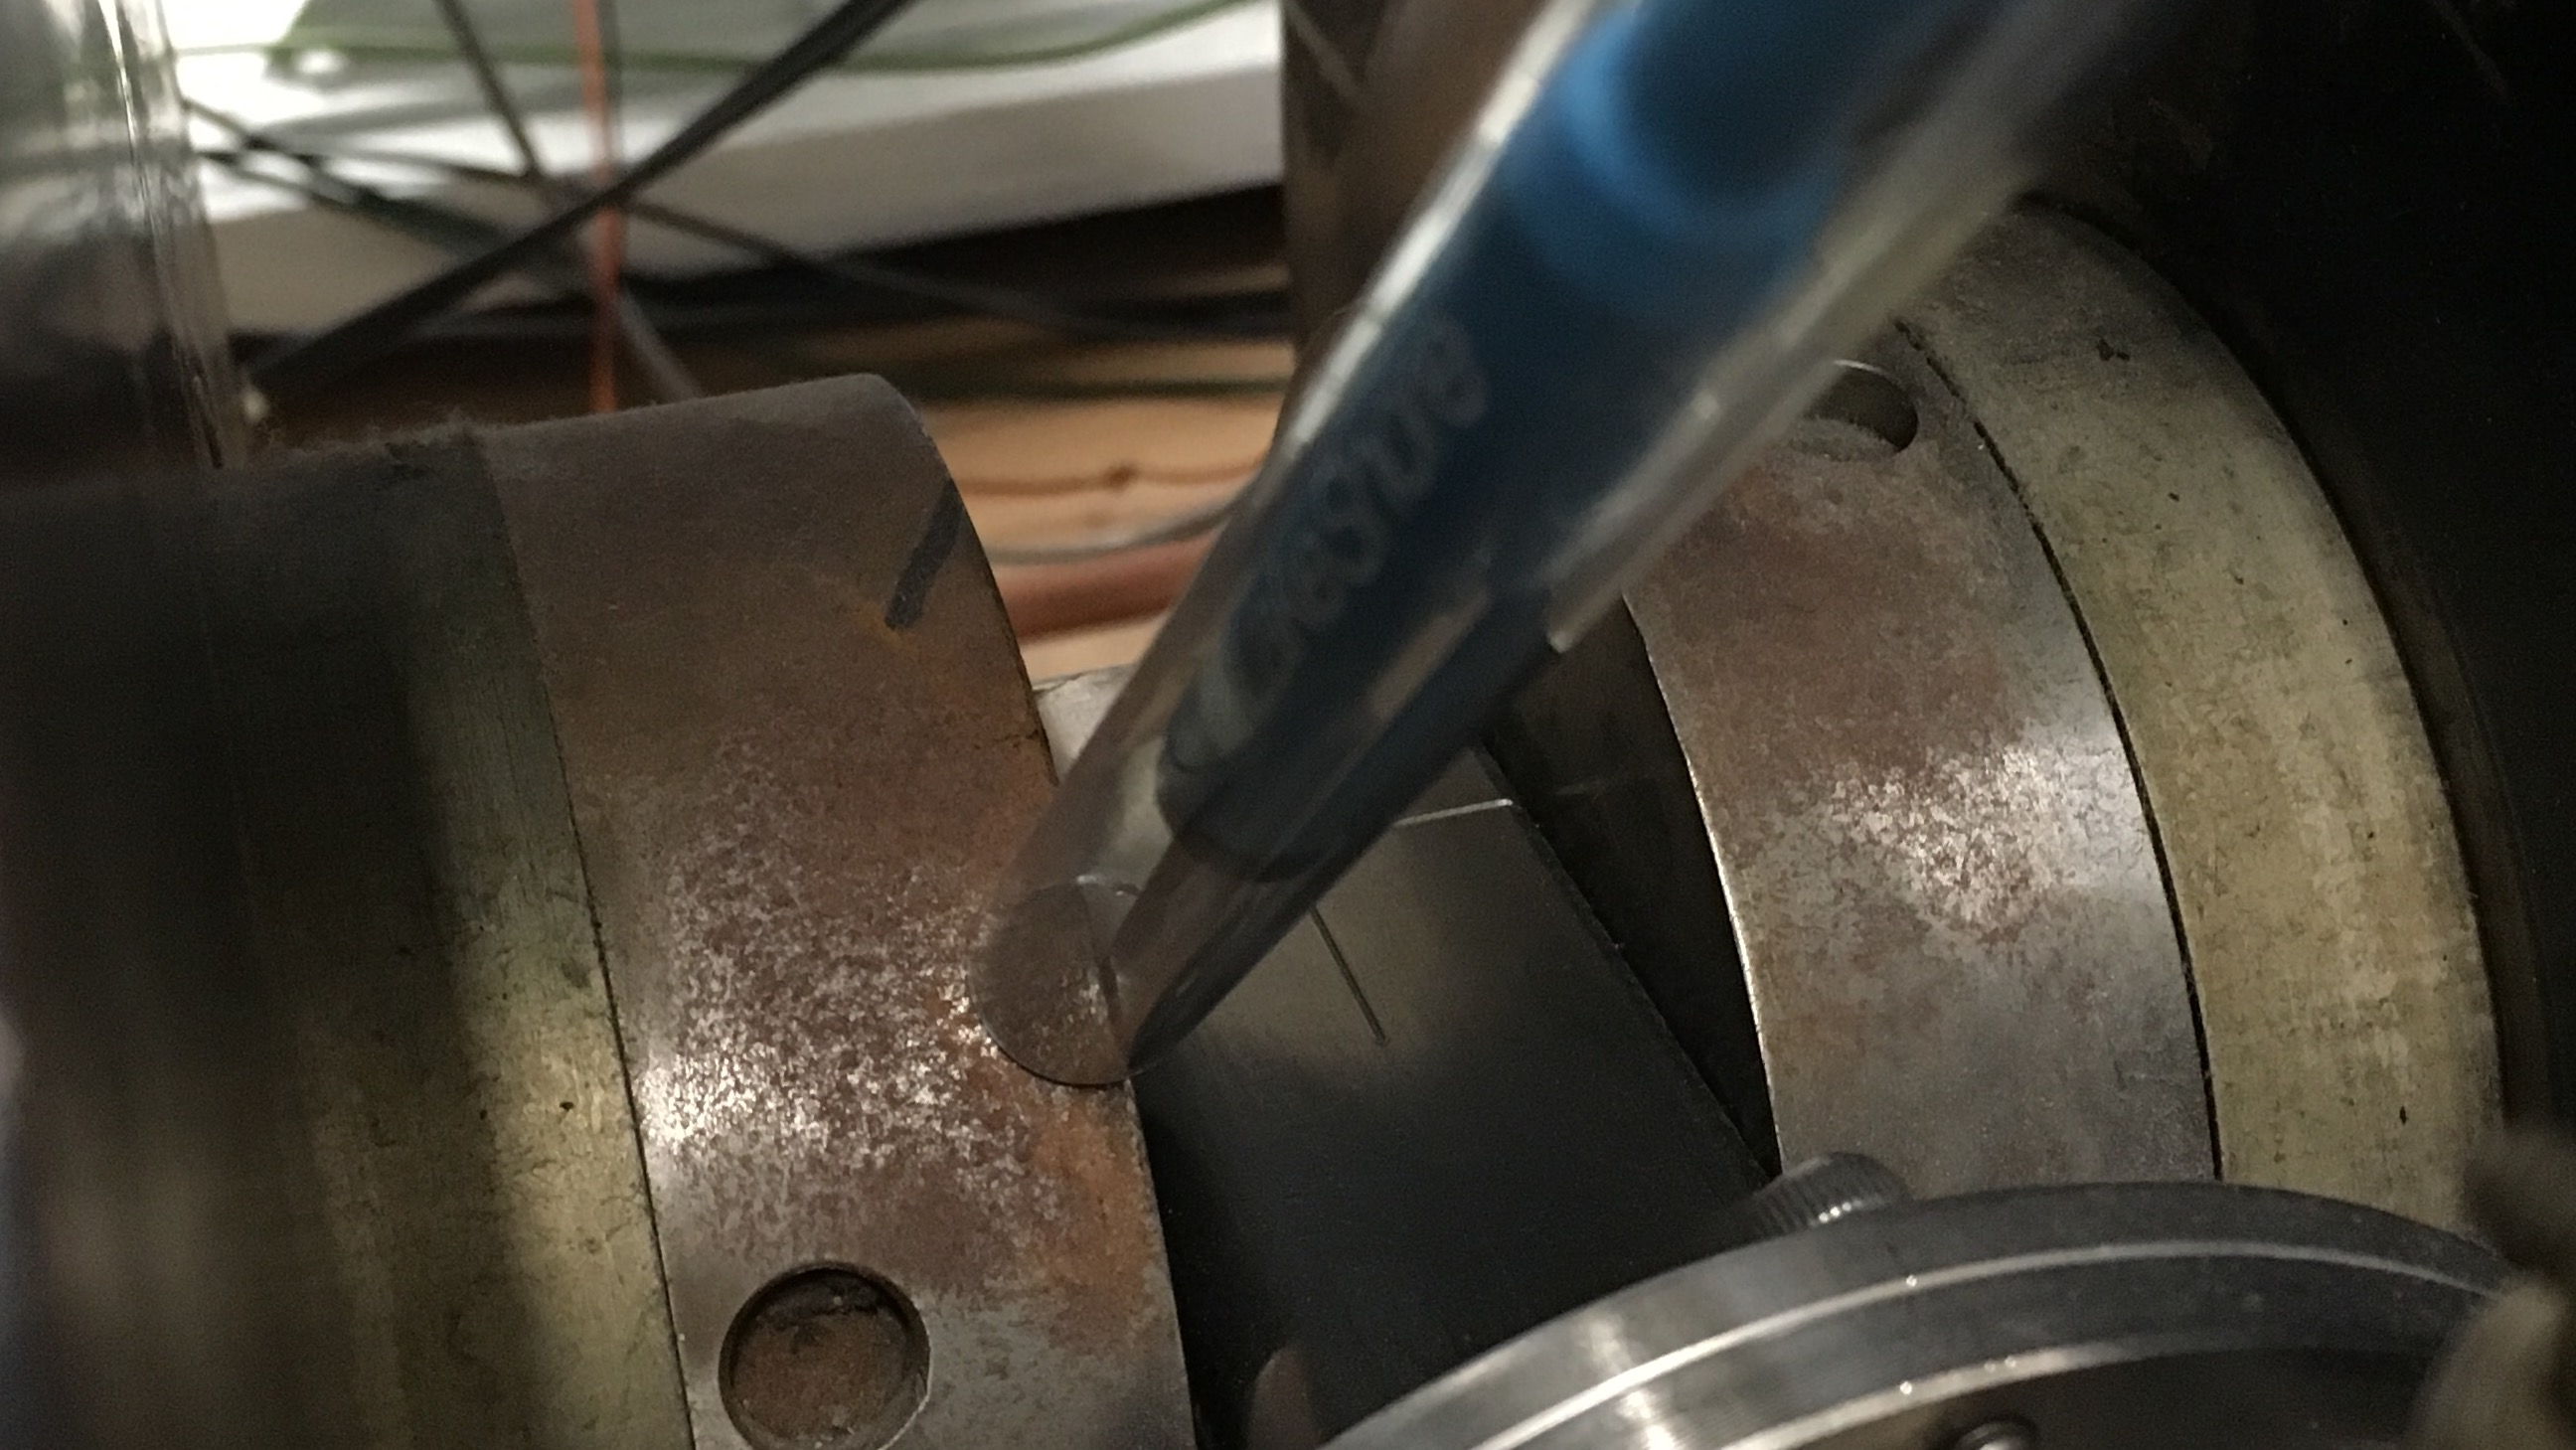
\includegraphics[width=\linewidth,keepaspectratio]{images/SHEimageGaussProbe.jpg}}
  \caption{Gauss Probe Close-up\\ \href{http://experimentationlab.berkeley.edu/sites/default/files/images/SHEimageGaussProbe.jpg}{Click here to see larger picture}}\label{fig:GaussProbe.jpg}
\endminipage\hfill
\minipage[t]{0.33\linewidth}
  
\includegraphics[width=\linewidth,keepaspectratio]{images/empty.png}
\endminipage
\end{figure}

\begin{figure}[H]
\captionsetup{justification=centering}
\minipage[t]{0.219\linewidth}
  \href{http://experimentationlab.berkeley.edu/sites/default/files/images/Magnet_Backside_Polepieces_Crop_3307.jpg}{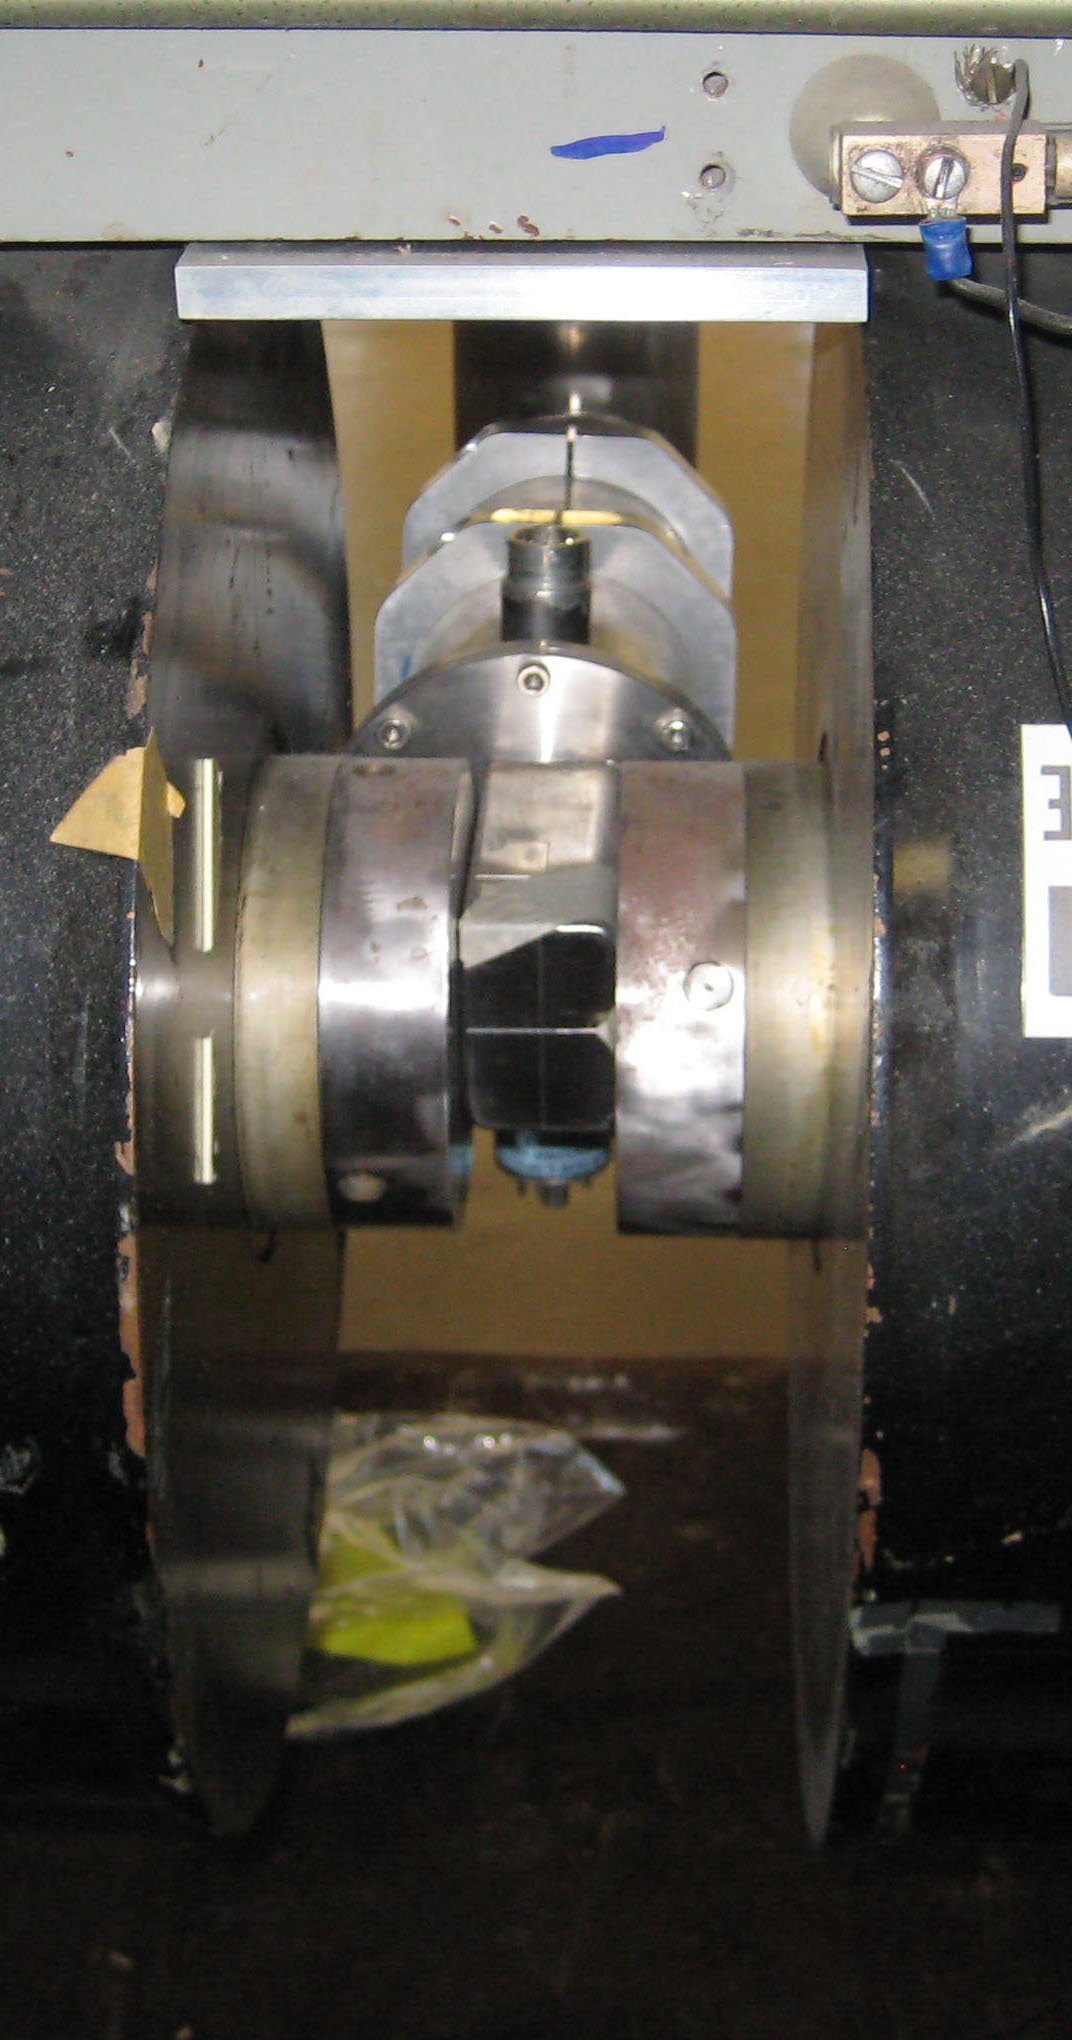
\includegraphics[width=\linewidth,keepaspectratio]{images/Magnet_Backside_Polepieces_Crop_3307.jpg}}
  \caption{Chamber Backside in Magnet \\ \href{http://experimentationlab.berkeley.edu/sites/default/files/images/Magnet_Backside_Polepieces_Crop_3307.jpg}{Click here to see larger picture}}
  \label{fig:Magnet_Backside_Polepieces_Crop_3307.jpg}
\endminipage\hfill
\minipage[t]{0.160\linewidth}
  \href{http://experimentationlab.berkeley.edu/sites/default/files/images/SHE_LN-2_Crop_3542.jpg}{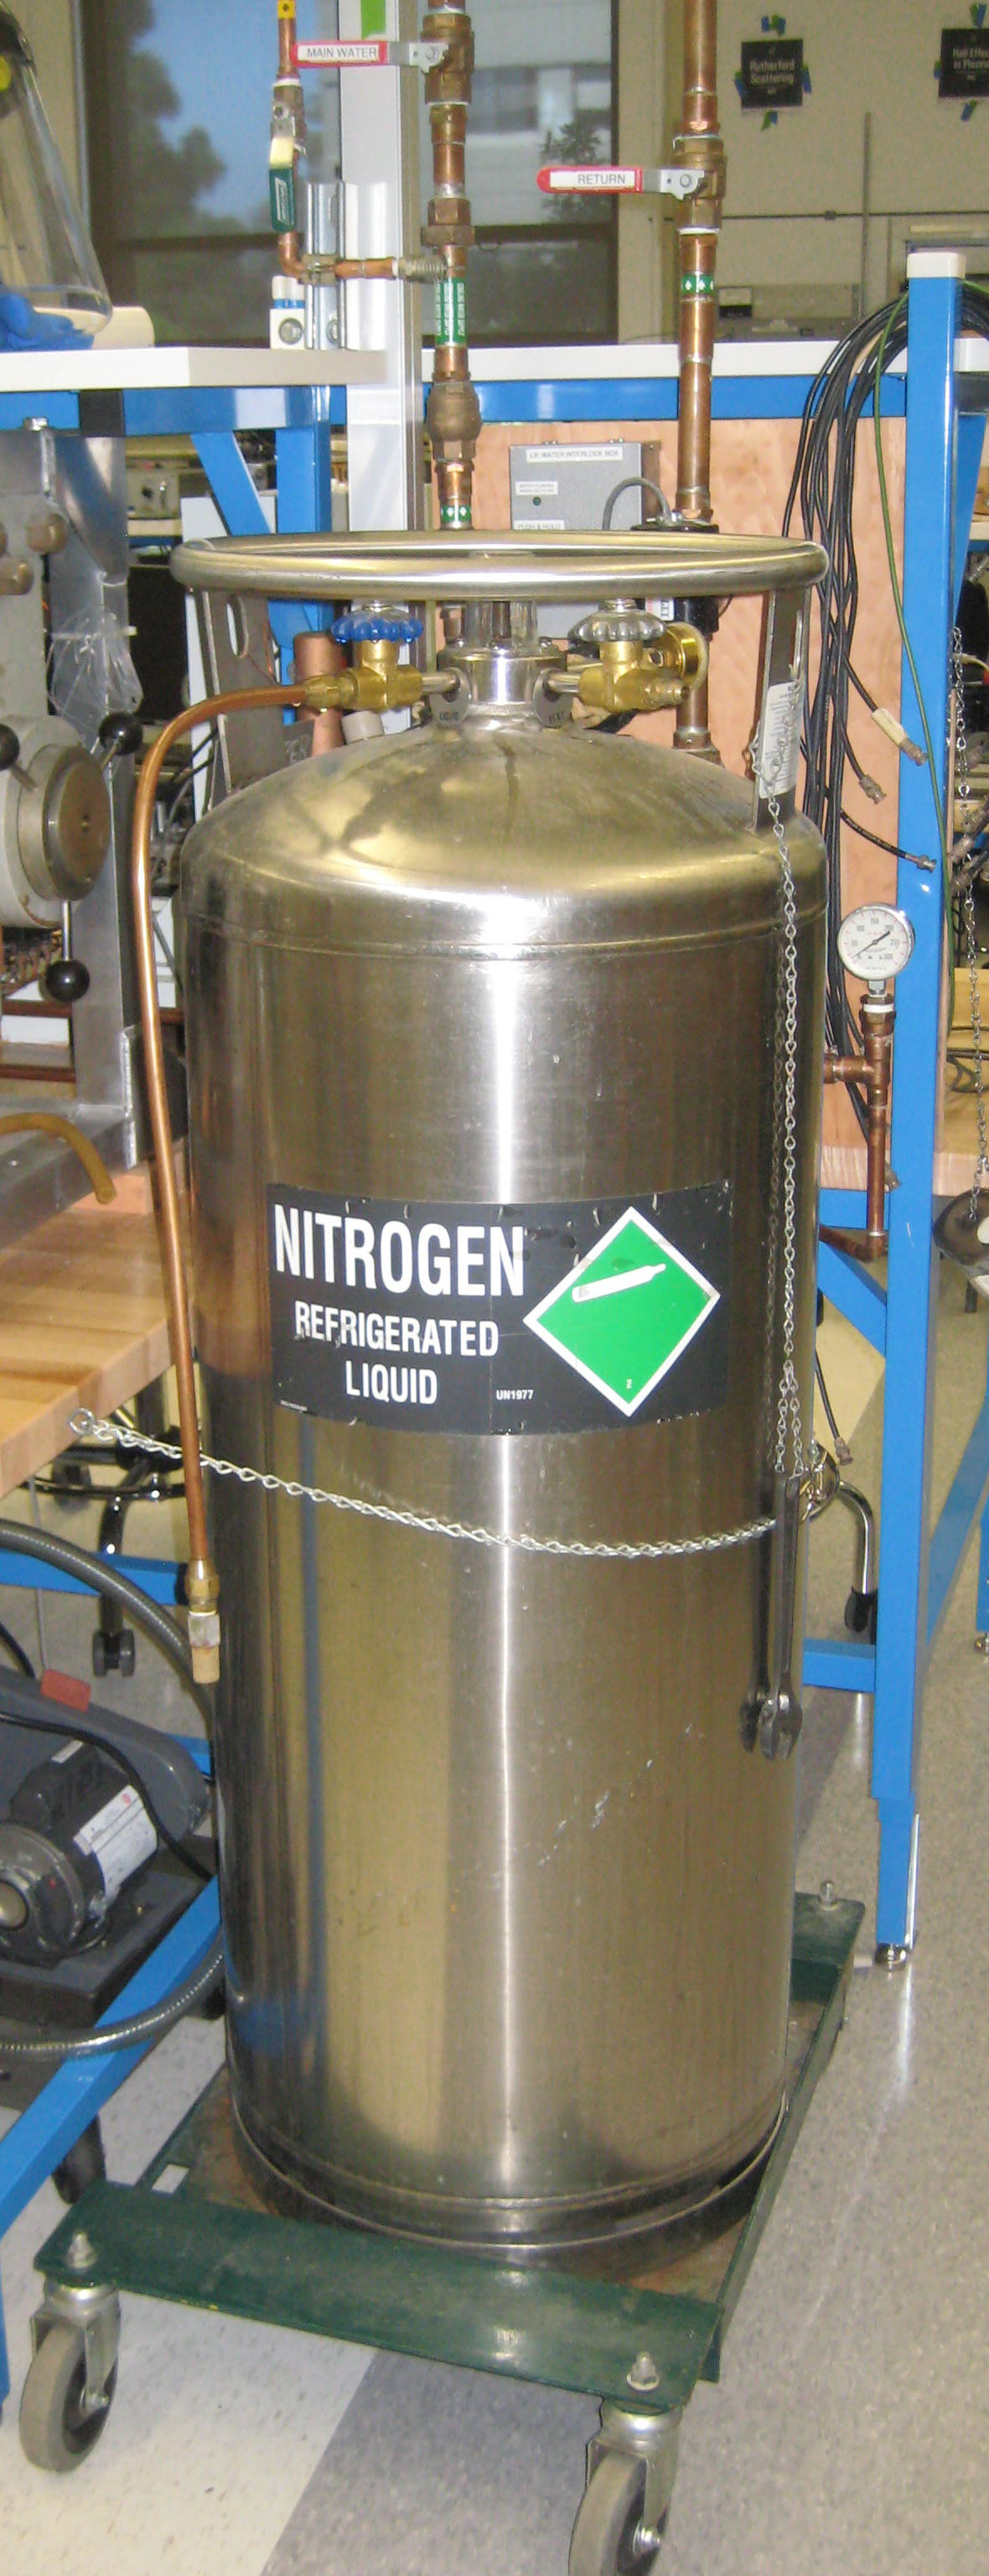
\includegraphics[width=\linewidth,keepaspectratio]{images/SHE_LN-2_Crop_3542.jpg}}
  \caption{Liquid Nitrogen Tank \\
  \href{http://experimentationlab.berkeley.edu/sites/default/files/images/SHE_LN-2_Crop_3542.jpg.jpg}{Click here to see larger picture}}
  \label{fig:SHE_LN-2_Crop_3542.jpg}
\endminipage\hfill
\minipage[t]{0.308\linewidth}
  \href{http://experimentationlab.berkeley.edu/sites/default/files/images/SHE_Water_Crop_3544.jpg}{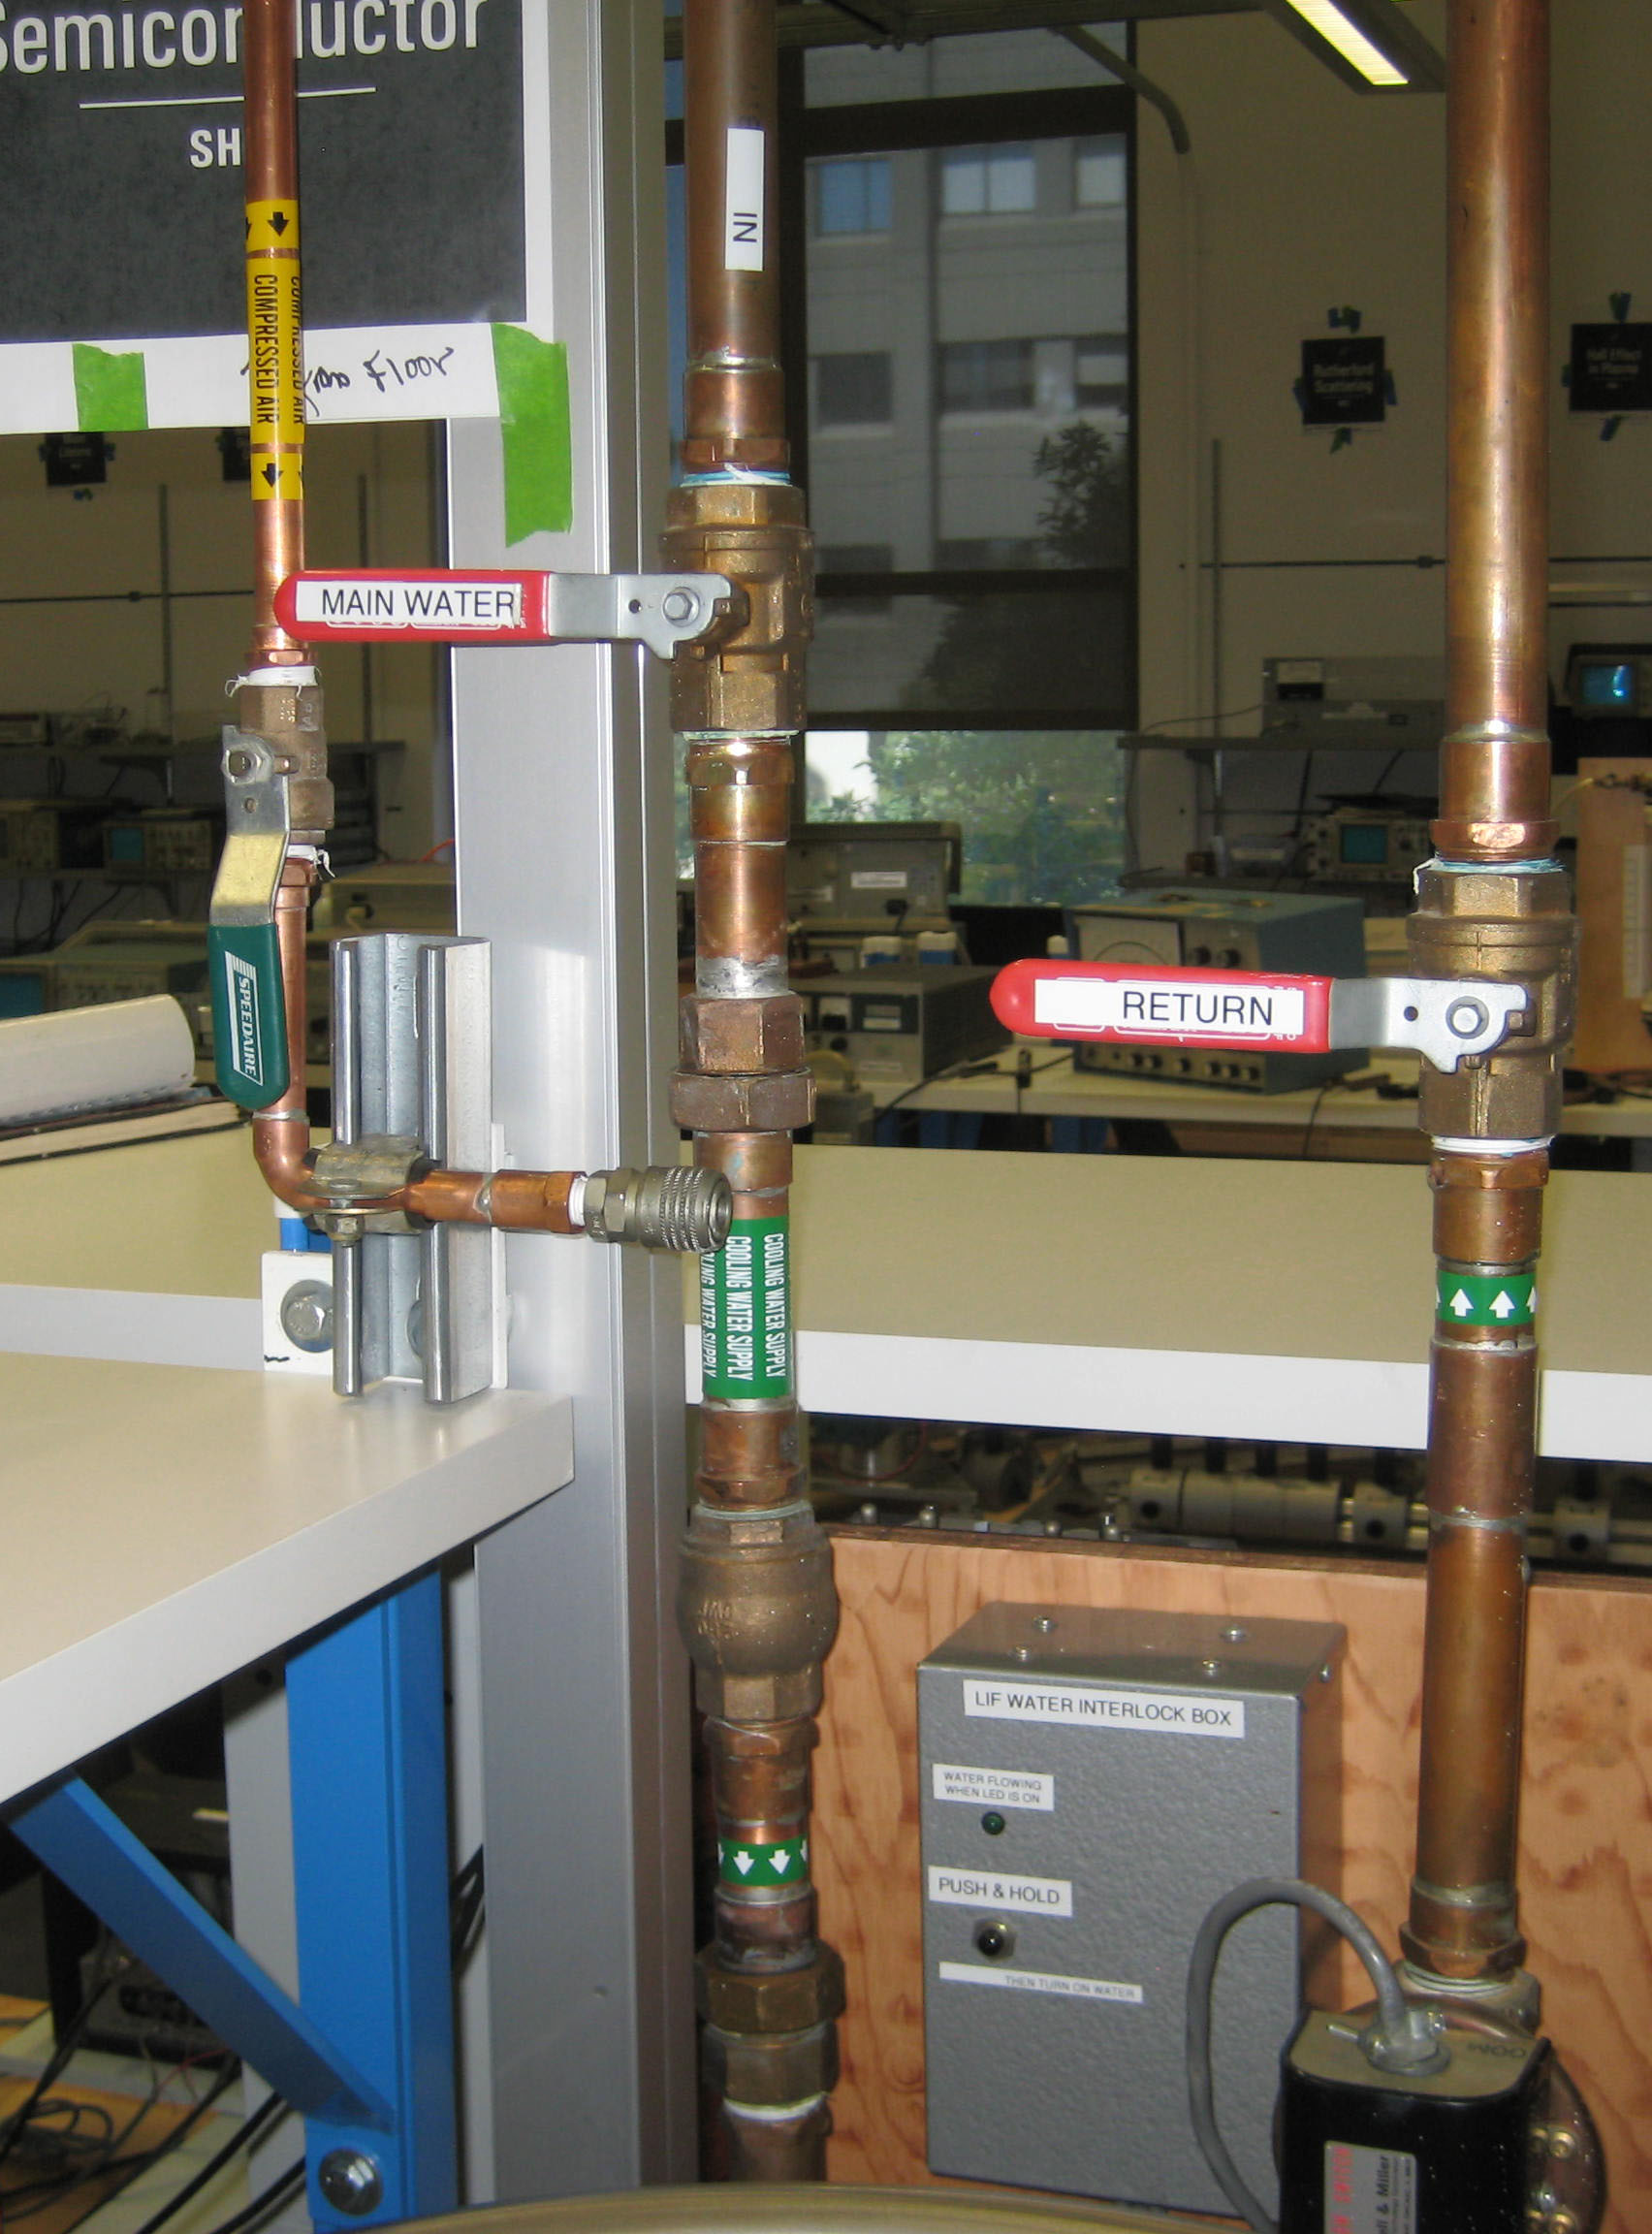
\includegraphics[width=\linewidth,keepaspectratio]{images/SHE_Water_Crop_3544.jpg}}
  \caption{Water Control valves and interlock box \\ \href{http://experimentationlab.berkeley.edu/sites/default/files/images/SHE_Water_Crop_3544.jpg}{Click here to see larger picture}}\label{fig:SHE_Water_Crop_3544.jpg}
\endminipage\hfill
\minipage[t]{0.294\linewidth}
  \href{http://experimentationlab.berkeley.edu/sites/default/files/upimages/5_eye-wear-face.jpg}{
\includegraphics[width=\linewidth,keepaspectratio]{images/5_eye-wear-face.jpg}} 
  
  \textbf{Wear Your Eye Safety Glasses \\ Liquid Helium danger}
  \label{fig:5_eye-wear-face.jpg}
\endminipage
\end{figure}

\section{Before the 1st Day of Lab}

\signatures \hyperlink{Hall Coefficient and Van der Pauw Method}{1} \hyperlink{Apparatus and Procedures}{2} \hyperlink{Extrapolating Data}{3} \hyperlink{Electron or Hole Concentrations}{4}

\begin{enumerate}
    \item \emph{\textbf{Note: In order to view the private Youtube videos hosted by the university, you must be signed into your berkeley.edu Google account.}}\\
    View the \href{http://youtu.be/7JYq1rRl6Xk}{\textbf{Hall Effect In a Semiconductor Video}}.

    \item Read before handling of Cryogenics: Read the Cryogenic Liquids information from the campus Environmental Health and Safety (EH\&S) department \href{http://experimentationlab.berkeley.edu/sites/default/files/images/77cryogenic.pdf}{\textbf{Cryogenic Liquids}}.

    \item Last day of the experiment please fill out the \href{\ExperimentEvaluation}{\textbf{Experiment Evaluation}}

\end{enumerate}

\noindent\textbf{Suggested Reading:}

\begin{enumerate}
    \item Melissinos, Adrian. ``\href{http://physics111.lib.berkeley.edu/Physics111/Reprints/SHE/SHE\_Melissinos\_properties\_of\_semiconductors\_pg\_80-98\_1966.pdf}{\textbf{\textbf{The Hall Effect and Properties of Semiconductors}.}}'' \emph{Experiments in Modern Physics,} pp. 80-98. Academic Press (1966).

    \item A short description of the Hall Effect. \href{http://physics111.lib.berkeley.edu/Physics111/Reprints/SHE/24-Haller.pdf}{\textbf{E. Haller Article}}

    \item ``Proof of the Van Der Pauw Theorem'' \href{http://experimentationlab.berkeley.edu/node/105}{\textbf{\textbf{Van Der Pauw Theorem}}}

    \item \href{http://physics111.lib.berkeley.edu/Physics111/Reprints/SHE/19-Four\_Wire\_Measurement.pdf}{\textbf{Four Wire Measurements}}

    \item The ``\href{http://physics111.lib.berkeley.edu/Physics111/Reprints/SHE/Semiconductor\%20Materials\%20Notes\%20MSE\%20223\%20Haller.pdf}{\textbf{Semiconductor Materials, Lecture Notes for MSE 223}}'' by E. E. Haller, Department of Materials Science and Engineering, University of California Berkeley.\textbf{You should search these MDE 223 notes for what you need.}

    \item \href{\LabReprints}{\textbf{\textbf{Physics 111-Lab Library site}}}

\end{enumerate}

More \hyperref[sec:References]{References}

\textbf{If you only read one reference, it is best to read Melissinos. It does a great job of explaining the physics. Section 3.3 on the Hall Effect will be vital during analysis when finding the Hall Voltage and extrapolating the conductivity values from the extrinsic region to the point where $T = T_{0}$. It will also shed some light on the concentrations of holes and electrons at the transition point.}

You should keep a laboratory notebook. The notebook should contain a detailed record of everything that was done and how/why it was done, as well as all of the data and analysis, also with plenty of how/why entries. This will aid you when you write your report.

\section{Objectives}

\begin{itemize}
    \item Investigating electrical conduction mechanisms in doped germanium with the Hall effect

    \item Demonstrating the Hall effect in doped germanium.

    \item Measuring the Hall voltage as a function of the current and magnetic field at room temperature.

    \item Determining the sign, density and mobility of charge carriers at room temperature.

    \item Measuring the Hall voltage as a function of sample temperature

    \item Determining the inversion temperature; differentiating between extrinsic and intrinsic conduction in the case of p-doped germanium.

\end{itemize}

\section{Useful Definitions}

\textbf{Conduction Band}

A Conduction band is a region in energy space (collection of different energy levels) where the lowest energy range of vacant electronic states resides and where charge carriers (electrons or holes) can move freely through a material.

\textbf{Conductor}

A conductor is a type of material in which charge carriers (effectively electrons or holes) can be made to flow with arbitrarily small voltages. The reasoning behind a conductors ability to move charge carriers with little resistance is rooted in quantum mechanical explanations and how electrons are arranged around the nuclei of atoms. The electron acts as both a wave and a particle, constraining its placement to distinct zones around the nucleus referred to as "shells" and "subshells". When an electron has enough energy to excite to higher energy states, it has the potential to break away from the force binding it to the atom and comprise part of an electric current throughout the immediately surrounding medium. A conductor is comprised of an atomic material that when an arbitrarily small voltage and thus potential is applied to it, it can easily liberate its electrons from their binding nuclei as they are not tightly bound.  The conducting material can be characterized as having a partially filled conduction band and, hence, no gaps between the highest occupied and the lowest unoccupied electronic states. Common examples of conductors are copper and iron.

\textbf{Electron Concentration}

is the number of electrons per unit volume in the conduction band of the material.

\textbf{Extrinsic material}

This is a type of impure semiconductor that has been ``doped'' in order to enhance its conductivity. There are two different types of extrinsic semiconductors: \emph{p-type} and \emph{n-type}. If a ``dopant'' atom is added to the lattice it will draw electrons from the valence band and is referred to as an ``\emph{acceptor''}. As more acceptors are added to the lattice, the number of holes will begin to exceed the number of negative charge carriers, eventually leading to a p-type (positive type) semiconductor. N-type semiconductors have a large number of\emph{ donors,} ``dopant'' atoms that donate electrons to the conduction band.

\textbf{Hall coefficient}

is a parameter that measures the magnitude of the Hall Effect in the sample. It has units of $\Omega$m/Tesla. (Contrast this with \emph{\textbf{resistivity}}, which has units of $\Omega$m.) The Hall coefficient is defined as $R_{H} = E/JB $  where $E$, $J$, and $B$ are the magnitudes of the electric field, the current density, and the magnetic field, respectively (It should be noted that in our experimental setup these three vectors are mutually perpendicular). A table of various element's resistivity and respective Hall Coefficient can be found in this \href{http://experimentationlab.berkeley.edu/sites/default/files/SHE/tableforRH.png}{\textbf{link}}.

\textbf{Hall effect}

is a phenomenon that occurs when a conductor or semiconductor carrying a current is placed in a magnetic field perpendicular to the current. This causes the charge carriers in the conductor to be deflected by the magnetic field and give rise to an electric field, due to the induced voltage by the separation of positive and negative carriers, known as the Hall field. This field is perpendicular to both the current and the magnetic field. The Hall Field can point along either direction of the axis it resides on. Note that, at sufficient temperature, the net current in a semiconductor is made up of counteracting currents of p-type and n-type carriers.

\textbf{Hall field}

is an electric field perpendicular to the direction of current flow generated by the Hall effect.

\textbf{Hall voltage}

is the potential difference across the semiconductor that is produced by the Hall field. This is the voltage which is exactly enough to compensate for the deflection of charge carriers by the magnetic field, so that the net current perpendicular to the applied voltage is zero.

\textbf{Hole}

is an effective positively charged ``empty state''. An electron hole is the lack of an electron in a position where one could exist in an atom or atomic lattice. If an electron is excited to a higher state then it leaves behind a hole in its old state.In our case it refers to the absence of an electron from the valence band. A good visual tool is to imagine the hole as a bubble in water, where the water is a sea of electrons in various surrounding energy levels. The description of current in terms of the motion of positively charged holes rather than negatively charged electrons is convenient and accurate when describing a material with an almost filled conduction band.

Hole conduction in a valence band can be explained by the following analogy. Imagine a row of people seated in an auditorium, where there are no spare chairs. Someone in the middle of the row wants to leave, so he jumps over the back of the seat into an empty row, and walks out. The empty row is analogous to the conduction band, and the person walking out is analogous to a free electron.

Now imagine someone else comes along and wants to sit down. The empty row has a poor view; so he does not want to sit there. Instead, a person in the crowded row moves into the empty seat the first person left behind. The empty seat moves one spot closer to the edge and the person waiting to sit down. The next person follows, and the next, et cetera. One could say that the empty seat moves towards the edge of the row. Once the empty seat reaches the edge, the new person can sit down.

In the process everyone in the row has moved along. If those people were negatively charged (like electrons), this movement would constitute conduction. If the seats themselves were positively charged, then only the vacant seat would be positive. This is a very simple model of how hole conduction works.

In reality, due to the crystal structure properties, the hole is not localized to a single position as described in the previous example. Rather, the hole spans an area in the crystal lattice covering many hundreds of unit cells. This is equivalent to being unable to tell which broken bond corresponds to the ``missing'' electron.

Instead of analyzing the movement of an empty state in the valence band as the movement of many separate electrons, a single equivalent imaginary particle called a ``hole'' is considered. In an applied electric field, the electrons move in one direction, corresponding to the hole moving in the other. If a hole associates itself with a neutral atom, that atom loses an electron and becomes positive. Therefore, the hole is taken to have positive charge of +e, precisely the opposite of the electron charge.

\textbf{Hole concentration}

is the number of holes (positive carriers) per unit volume in the conduction band of the material.

\textbf{Intrinsic material}

This is a type of pure Semiconductors in which its properties are solely based off of the material itself (as it has not been doped). Here, the number of electrons (negative carriers) in the conduction band equal the number of holes (positive carriers) in the valence band. These semiconductors are also known as i-types.

\textbf{Insulator}

An insulator is a type of material material in which, unlike conductors, charge carriers cannot be made to flow with low voltages. Using the quantum mechanical description of periodic solids, insulators are characterized by having completely filled valence bands, and large energy gaps to the lowest-lying unoccupied conduction bands.

\textbf{Drift mobility}

is the drift velocity per unit applied electric field, $\mu_d = \nu_d/ E$.

\textbf{Drift velocity}

is the average velocity in the direction of an applied electric field of the all conducting charge carriers in the sample.

\textbf{Lorentz force}

is the force, $\vec{F} = q(\vec{\nu} \times \vec{B}) $ which a moving charge experiences when subjected to a magnetic field. Here, $\vec{B}$ is the magnetic field, $\vec{\nu}$ is the velocity of the carrier, and $q$ its charge.

\textbf{N-type material}

N-type semiconductors have a larger electron concentration than hole concentration. The phrase 'n-type' comes from the negative charge of the electron. In n-type semiconductors, electrons are the majority carriers and holes are the minority carriers. N-type semiconductors are created by doping an intrinsic semiconductor with donor impurities (or doping a p-type semiconductor as done in the making of CMOS chips). A common dopant for n-type silicon is phosphorus. In an n-type semiconductor, the Fermi level is greater than that of the intrinsic semiconductor and lies closer to the conduction band than the valence band.

\textbf{P-type material}

As opposed to n-type semiconductors, p-type semiconductors have a larger hole concentration than electron concentration. The phrase 'p-type' refers to the positive charge of the hole. In p-type semiconductors, holes are the majority carriers and electrons are the minority carriers. P-type semiconductors are created by doping an intrinsic semiconductor with acceptor impurities (or doping an n-type semiconductor). A common p-type dopant for silicon is boron. For p-type semiconductors the Fermi level is below the intrinsic Fermi level and lies closer to the valence band than the conduction band.

\textbf{Resistivity}

is a material parameter that is a measure of the resistance to current. The resistivity is defined as the resistance of the sample times the cross sectional area of the sample divided by the length of the sample, $\rho = RA/l$. The resistivity has units of $\Omega$m and it is inversely proportional to the conductivity of the sample, $\sigma = 1/\rho$.

\textbf{Semiconductor}

is a nonmetallic element (e.g. Si or Ge) that contain both electrons and holes as charge carriers in contrast to an enormous number of electrons only as in metals. Electron and hole concentrations in a semiconductor are generally many orders of magnitude less than those in metals, thus leading to much smaller conductivity. Although technically they are considered insulators, they posses the characteristic of barely insulating, this simply means that the filled conduction band lies very close to the valence band. Semiconductors can be deliberately modified through patterned doping to produce complex, compact, and reliable electronic devices.

\checkpoint{Hall Coefficient and Van der Pauw Method}{Explain to Professor or GSI what the Hall Coefficient is. Explain what the Van der Pauw method is, including why it's useful.}

\section{Introduction}

The applications of modern semiconductors are immeasurable; they allow us to construct microscopic transistors used in logic gates that act as on or off switches for digital circuitry. Differing semiconductor materials possess different properties, each suitable for the nature of their use. One such property is their ability to conduct under various surrounding environmental conditions. These semi-conductors materials are classified on the carrier concentrations as well as their motions throughout the semiconductor when influenced by external electromagnetic fields. Thus, due to the nature of their scale, these modern building blocks rely heavily on the purity of their states. The semiconductor industry relies on mature technologies for the creation of high purity semiconductors and for their quantitative characterization prior to their use in manufacturing. One important characterization tool in the measurement of the Hall effect to measure mobilities and carrier concentrations in a given semiconductor material. In this experiment, we will make such measurements, observing the Hall effect for one semiconductor sample using the common Van der Pauw technique. The temperature dependence of the Hall coefficient and resistivity will allow us to distinguish between p-type and n-type samples, and to calculate the electron and hole mobilities and concentrations. The maximum sample current you should use is 0.9 mA. You should try a variety of sample currents, probably in order of magnitudes. ( 1 microamp to 10 milliamps)

\section{Preliminary Concepts}

The electrical properties of conductors and dielectrics are easy to understand and straightforward to measure (e.g. a simple confirmation of Ohm's law). In contrast, the properties of semiconductors fall in between these two extremes and require some knowledge of condensed-matter quantum physics to understand.

Recall some simple concepts from the quantum description of an isolated atom. Electrons in an atom are regarded as occupying quantized single-electron energy levels (at least in the ``independent particle approximation''). If an atom is in its ground state, its N electrons will occupy the N lowest energy (i.e. most tightly bound) states available around that atom's nucleus. Electrons can be promoted to one of the infinite number of unoccupied energy levels (bound or unbound) if sufficient energy and a proper means of excitation are provided (e.g. barring selection rules).

\begin{figure}[h]
    \centering
    \href{http://experimentationlab.berkeley.edu/sites/default/files/images/SHEimage016.gif}{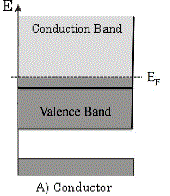
\includegraphics[width=0.25\linewidth,keepaspectratio]{images/SHEimage016.png}}
    \href{http://experimentationlab.berkeley.edu/sites/default/files/images/SHEimage017.gif}{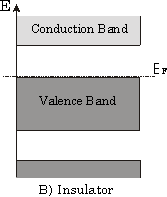
\includegraphics[width=0.25\linewidth,keepaspectratio]{images/SHEimage017.png}}
    \href{http://experimentationlab.berkeley.edu/sites/default/files/images/SHEimage018.gif}{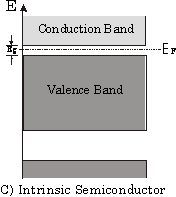
\includegraphics[width=0.25\linewidth,keepaspectratio]{images/SHEimage018.png}}
    \caption{Energy-band diagrams for A) Conductor, B) Insulator, C) Intrinsic Semiconductor. The dark shaded gray parts correspond to the filled states. The lightly shaded gray parts corresponded to unoccupied states. $E_{F}$ is the Fermi energy and $E_{g}$ is the band gap energy.}
    \label{fig:EnergyBandDiagrams}
\end{figure}

In a solid, however, the atoms are packed closely together, and the strong mutual influence of neighboring atoms forces one to treat electron quantum levels as being delocalized throughout the solid rather than as being localized around just a single nucleus. In this situation, the energy spectrum now consists of bands of allowed energies, each of which arises gradually from the isolated atomic states as atoms are brought together to their small spacings in the solid. These energy bands consist of a continuum of energies for electronic states which differ in momentum (or, rather, ``quasi-momentum''), and are separated from each other by energy gaps which are energy ranges which electrons in the solid cannot possess.

Further, under typical conditions, the electrons in a solid are deep in the regime of quantum degeneracy, which we can determine as follows. At zero temperature, electrons in the solid would occupy sequentially all the lowest energy states up to an energy, the Fermi energy. At temperatures $T$ such that $E_F = k_B T$, where $k_B$ is the Boltzmann constant, the distribution of electrons is modified slightly, with some electrons right near the Fermi energy actually being thermally promoted to energy levels above the Fermi energy, with this redistribution all happening within about $k_B T$ of the Fermi energy.

Now we may understand the quantum-mechanical distinction between conductors, insulators, and semiconductors (Figure \ref{fig:EnergyBandDiagrams}). In a conductor, the Fermi energy lies within an allowed energy band. Because of this, electrons can respond to minutely small electric fields by small redistributions among nearby energy levels so that an electrical current flows. By contrast, in an insulator, the valence band (the highest energy band which is occupied) is completely filled, and is separated by a large energy gap from the conduction band (the lowest energy band which is not fully occupied). Since large energies are now needed to redistribute electrons in such a material, small electric fields will no longer induce electronic motion, and hence no current will flow.

As shown in Figure \ref{fig:EnergyBandDiagrams}c, the situation in a semiconductor is between that of a conductor and an insulator. While a semiconductor is, strictly speaking, an insulator, it is insulating only due to a very small energy gap. By ``small,'' we mean the gap is on the order of the thermal energy $k_B T$. For such a material, therefore, there exists a small concentration of empty states (holes) in the valence band and of filled states (electrons) in the conduction band due to thermal excitation. As such, a semiconductor has a small, strongly temperature dependent, conductivity.

Furthermore, the small energy gap makes the electronic properties of a semiconductor highly susceptible to ``doping,'' i.e. the controlled introduction of a small density of electronic levels at energies \emph{within} the intrinsically void energy gap by the mixing of impurity atoms within a semiconductor. These impurity atoms serve either to add extra filled electron levels at energies near the conduction band edge, thereby providing a surplus of electrons into the conduction band, or to add extra unfilled levels at energies near the valence band edge, thereby providing a surplus of holes into the valence band. The former situation creates an n-type semiconductor, in which the majority of charge carriers are negatively charged, while the latter creates a p-type semiconductor, in which the majority of charge carriers are positively charged. Undoped semiconductors are called \emph{intrinsic}, while doped ones are called \emph{extrinsic}. In an intrinsic semiconductor, the densities of free electrons and holes are equal, while in extrinsic semiconductors, as explained above, these densities are unequal.

\begin{figure}[h]
    \centering
    \href{http://experimentationlab.berkeley.edu/sites/default/files/images/SHEimage023.gif}{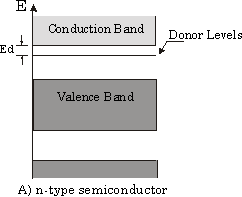
\includegraphics[width=0.33\linewidth,keepaspectratio]{images/SHEimage023.png}}
    \href{http://experimentationlab.berkeley.edu/sites/default/files/images/SHEimage024.gif}{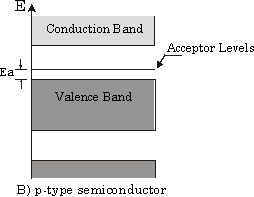
\includegraphics[width=0.33\linewidth,keepaspectratio]{images/SHEimage024.png}}
    \caption{Energy band diagrams for extrinsic type semiconductors. The N-type semiconductor in a) contains occupied donor levels located at energy Ed below the conduction band. Electrons in these levels are easily excited into the conduction band. P-type semiconductors b) have vacant acceptor levels at energy Ea above the valence band. Electrons from the top of the valence band can be easily excited into these levels. The dark shaded gray corresponds to filled states and lightly shaded gray corresponds to unoccupied levels.}
\end{figure}

Differences between conductors and semiconductors can be quantified through the resistivity $\rho$ of each material. Resistivity is a bulk quantity defined as $\rho = E/J$, where $E$ is the electric field (measured in Volt/meter) and $J$ the current density (measured in Ampere/meter$^2$). The SI unit of resistivity is thus the Ohm-meter. As an example of properties for a metal, the resistivity of copper is near $2 \times 10^{-8} \Omega$m at room temperature, increasing slowly (at a relative rate of $4 \times 10^{-3}$/K in copper) as temperature increases. A remarkable thing about conduction in metals is that the electrons forming the current move at an extremely slow \emph{net drift velocity} ($\sim$10 micron/s) on top of a random thermal motion at much higher speeds ($\sim 10^6$ m/s). The value of the slow drift velocity can be estimated by considering how fast electrons at a density of $\sim 10^{29}$/m$^3$ (say one per copper atom) would have to move in a typically-sized conductor to give a typical current (e.g. 1 ampere in a mm$^{2}$ cross section).

By contrast, a semiconductor such as silicon has fewer charge carriers, ($10^{-16}$/m$^3$), a larger resistivity ($3 \times 10^3$ ohm-meters), and a \emph{negative} temperature coefficient of resistivity ($-10^{-3}$/K). The resistivity can be changed drastically by doping with other materials – typically decreasing from $3 \times 10^3$ to $10^{-3}$ ohm-m!

\section{Hall Effect and Van Der Pauw Technique}

To determine the electrical resistance of an object, one measures two quantities: the current run through the object and the voltage which arises due to the passage of that resistance. There are two typical ways for performing such measurements, either the simple but somewhat inaccurate two-probe technique, or the more cumbersome by more accurate four-probe technique. The difference between these two techniques is particularly pertinent when one wants to measure very small resistances. Using a two-probe technique, such as one usually does with an ohmmeter, current exits the device and runs in series across many resistive elements: the wires coming out of the ohmmeter, the substantial (fraction of an Ohm) contact resistance between the ohmmeter probes and the resistor, then the resistor, more contact resistance, and more wire. The voltage is then measured in the ohmmeter across the \emph{entire} chain of resistors, meaning that the small resistance you were trying to measure is swamped by the extraneous contact resistances. This difficulty is overcome by using a four-probe technique. One device is used to generate current, and run that current across contact resistances as well as the resistor you're trying to measure. Then a second \emph{high-input-impedance} device, i.e. one that draws very little current, is used to sample the voltage \emph{only across the resistor}, and is thereby insensitive to voltage drops due to contact resistance. Since the contact resistance for the \emph{voltage probes} is much smaller than the input impedance of the voltmeter, we obtain a genuine voltage measurement to use in our resistance determination. In this experiment, we will use several well-conceived measurement techniques to determine the resistivity and the Hall voltage across our semiconductor samples.

\subsection{Hall Effect}

\begin{figure}[h]
    \centering
    \href{http://experimentationlab.berkeley.edu/sites/default/files/images/SHEimage028.gif}{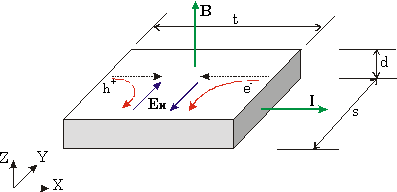
\includegraphics[width=0.5\linewidth]{images/SHEimage028.png}}
    \caption{Hall Effect Geometry}
    \label{fig:HallEffectGeometry}
\end{figure}

Consider a semiconductor sample placed in the magnetic field $B$ that is in the $z$-direction (refer to Figure \ref{fig:HallEffectGeometry}). Suppose we pass a current $I$ through that sample perpendicular to the magnetic field, say in the $x$-direction. Then the ``free'' electrons and ``holes'' in the sample experience a force given by the Lorentz equation,
\begin{equation}
    \vec{F}=q(\vec{\nu}\times\vec{B}) \quad [N]
\end{equation}
where $Q$ is the charge of free carriers and $ \vec{\nu} $ their velocity. This force deflects \emph{any} charge carriers towards in the positive y direction. If the charge carriers are predominantly electrons, this creates an excess negative charge on the $+y$ side of the semiconductor sample, and thus a positive charge on the $-y$ side. This charge distribution generates an electric field $ E_H $ (the Hall field) pointing in the $+y$ direction which (1) balances the Lorentz force so as to keep current flowing along the $x$-direction, and (2) yields a voltage difference $ V_H=sE_H $ (the Hall voltage, named after E.H. Hall who discovered this effect in 1879) across the sample of width \emph{s}. Considering the balance of forces on the charge carriers,
\begin{equation}
    \vec{F}=q(\vec{E}+\vec{\nu}\times\vec{B})=0 \quad [N]
\end{equation}
we see that
\begin{equation}
    E_H=\nu_xB_z \quad [V/\text{m}]
\end{equation}
Since $ I\propto qv_x $, we see that the sign of the Hall voltage $ V_H $ will depend on whether the charge carriers are predominantly negatively (electrons) or positively (holes) charged. Thus, by measuring the Hall voltage we can determine whether we have an n-type or p-type semiconductor.

Let us now consider how the velocity of charge carriers, as measured through the Hall effect, can be related to important parameters of the semiconductor sample. Suppose the charge carriers in our sample are the (negatively charged) electrons, i.e. our semiconductor is n-type. Taking into account the dimensions of the sample, the total current is related to the density of charge carriers \emph{n} and their drift velocity $ \nu_x $ as

\begin{equation}
    I=(-env_x)(sd) \quad [A]
\end{equation}
i.e. as the product of the current density $ J=-qn\nu_x $ and the cross-sectional area of the conductor. Recalling the relation of the Hall voltage, we obtain the following expression by which the electron density may be determined:

\begin{equation}
    V_H=-\frac{I_xB_z}{end} \quad [V]
\end{equation}
Using this definition, we also obtain the Hall coefficient $ R_H $ as

\begin{equation}
    R_H=\frac{E_H}{J_xB_z}=\frac{1}{en} \quad [\text{m}^3/C]
\end{equation}
We use these expressions if the Hall voltage $ V_H $ is negative. If $ V_H $ is positive, our sample is a p-type semiconductor, the current through which is carried by holes the density which, \emph{p}, is determined through

\begin{equation}
    V_H=\frac{I_xB_z}{epd} \quad [V]
\end{equation}
and obtain for the Hall coefficient $R_H = -1/ep$.

Finally, we note that the current through a semiconductor may be \emph{simultaneously} due both to electrons and to holes. To isolate the density of each, rather than just the overall charge-weighted carrier density, we must examine and interpret the dependence of the Hall voltage on temperature.

\subsection{Van Der Pauw Technique}

\begin{figure}[h]
    \centering
    \href{http://experimentationlab.berkeley.edu/sites/default/files/images/SHEimage052.gif}{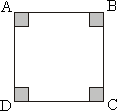
\includegraphics[width=0.3\linewidth]{images/SHEimage052.png}}
    \caption{Van der Pauw configuration}
    \label{fig:VanDerPauwConfiguration}
\end{figure}

A clever way of obtaining the Hall voltage and also the resistivity of the sample is the so-called Van der Pauw technique \href{http://experimentationlab.berkeley.edu/node/105}{\textbf{Van Der Pauw Theorem}} . Suppose we have a semiconductor sample containing four small contacts \emph{A}, \emph{B}, \emph{C}, and \emph{D} as shown in Figure \ref{fig:VanDerPauwConfiguration}. We will use these four contacts to variably drive currents and measure voltage drops, using, for example, the notation that $I_{AB}$ is the current driven from point A to point B, and that $V_{CD}$ is the voltage drop between points C and D (defined positive if the voltage at C is higher than at D). For each configuration of current flow and voltage measurement, we will measure the ``trans-resistance'' denoted as, for example, $R_{AB,CD} = V_{CD} / I_{AB}$. Four different measurement configurations will be used, as indicated by the table below:

Measurements indicated by the first two rows (e.g. current driven between adjacent points) will lead us to the resistivity, while those in the last two rows (e.g. current driven between non-adjacent points) lead to the Hall voltage. Starting with the Hall voltage, we simply use the last two sets of measured quantities to obtain the average trans-resistance $(R_{AC,BD} + R_{BD,CA})/2$. We use this quantity, along with a measurement of the magnetic field $B_z$, and of the sample dimensions to obtain the Hall coefficient, applying the formulae of equations 5 or 7 depending on the sign of the trans-resistance.

Determining the resistivity $\rho$ of the sample is somewhat more subtle. Leaving detailed derivations for Appendix A, we will make use of the Van der Pauw equation
\begin{equation}
\label{eq:VanDerPauwEquation}
    \exp \left(\frac{-\pi d}{\rho} R_{AB,CD} \right) + \exp \left(\frac{-\pi d}{\rho} R_{AD,CB} \right) = 1
\end{equation}
by which $\rho$ is implicitly determined (here $d$ is the sample depth, referring to Figure \ref{fig:HallEffectGeometry}). While this equation appears difficult to solve, one readily sees that all solutions with the same \emph{ratio} $R_{AB,CD} / R_{AD,CB}$ are trivially related to each other. Thus, we may write for the resistivity
\begin{equation}
\label{eq:Resistivity}
    \rho = \frac{\pi d}{\ln(2)} \cdot \frac{(R_{AB,CD}+R_{AD,CB})}{2} \cdot f \left( \frac{R_{AB,CD}}{R_{AD,CB}} \right)
\end{equation}
The only difficult part remaining is the determination of the function $f(x)$, a task which need be performed only once, and which is indeed already performed for us; the solution is graphed in Figure \ref{fig:FVersusResistanceRatio}. To a good approximation, we may take $f(x) = 1/\cosh(\ln(x)/2.403)$ (to better than 0.1\% for $x < 2.2$), and better than 1\% for $x < 4.3$). For the derivation of equations \eqref{eq:VanDerPauwEquation} and \eqref{eq:Resistivity} see Appendix A.

\begin{figure}[h]
    \centering
    \href{http://experimentationlab.berkeley.edu/sites/default/files/images/SHE76image003.jpg}{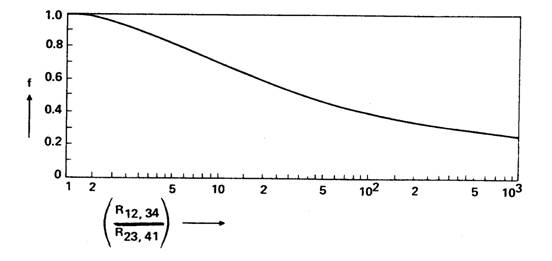
\includegraphics[width=0.7\linewidth]{images/SHE76image003.jpg}}
    \caption{The function $f$ versus the resistance ratio. This function is used to determine the resistivity of the sample. Here $R_{12,34}$ is equivalent to $R_{AB,CD}$ and $R_{23,41}$ is same as $R_{AD,CB}$. (This figure appears in ``Semiconductor Materials, Lecture Notes for MSE 223'' by E. E. Haller, Department of Materials Science and Engineering, University of California Berkeley.)}
    \label{fig:FVersusResistanceRatio}
\end{figure}

For good measure, once the above procedure has been completed, it is worthwhile to verify our experimental technique. Thus, we will make four more sets of measurements (just the reverse of the previous ones), indicated by the table below.

\begin{center}
    \begin{tabular}{l|l|l}
        Current  & Voltage  & Trans-resistance \\\hline
        $I_{BA}$ & $V_{DC}$ & $R_{BA,DC} = V_{DC} / I_{BA}$ \\\hline
        $I_{DA}$ & $V_{BC}$ & $R_{DA,BC} = V_{BC} / I_{DA}$ \\\hline
        $I_{CA}$ & $V_{DB}$ & $R_{CA,DB} = V_{DB} / I_{CA}$ \\\hline
        $I_{DB}$ & $V_{AC}$ & $R_{DB,AC} = V_{AC} / I_{DB}$
    \end{tabular}
\end{center}

Once again, we use these trans-resistances to determine the Hall voltage and the resistivity. The results of the two sets of measurements should obviously agree.

From measurements of the resistivity, we obtain the \emph{mobilities} of the charge carriers in our sample as follows:
\begin{equation}
    1/\rho = e \cdot (n\cdot\mu_n + p\cdot\mu_p)
\end{equation}
Here, $\mu_n$ is the electron mobility and $\mu_p$ the hole mobility. This equation is trivially adapted to samples in which the carriers are exclusively either electrons or holes. The charge carrier densities $n$ (electrons) and $p$ (holes) come from our Hall voltage measurements.

Finally, having experimentally determined the carrier concentrations and mobilities, we obtain their drift velocities, given as $\nu_{de} = \mu_n E$ for electrons and as $\nu_{dp} = \mu_p E$ for holes. In both expressions, $E$ is the magnitude of the electric field which drives the current.

In this experiment we are going to make measurements of Hall Voltage and sample resistivity as it varies with temperature. We will start with the sample at room temperature, around 320K. Adding liquid nitrogen, we will begin to cool down the sample. Below 240K we will add more liquid nitrogen to replace boil off. Once the system has reached the specified starting temperature, the computer automatically senses it. At this point the heater will start warming up the sample. Once this begins, it is not possible to change the starting and ending temperatures, except by stopping the experiment early. The computer will begin to record data every degree change as the temperature rises at 5K per minute. (These data should be preserved in the data file, even if the program is terminated early or even if the computer crashes.) The temperature controller (running autonomously) will stop heating the sample at 400K (the ending temperature), and computer will stop taking the data. We are going to stop at 400K to prevent the melting of the soldered contacts on the sample. (The contacts will begin to break down at 156° C and we want to stay below that point.) The contact points of the sample consist of Boron dopant covered by a Palladium layer which in turn is covered by a gold layer which is covered by an indium layer. Then, wires are pressed onto the indium contacts (see photo, below, of this process). These contacts are very delicate. Please do not touch them. If you think there is a problem with the mounted sample, ask for help from the staff.

\begin{figure}[h]
    \centering
    \href{http://experimentationlab.berkeley.edu/sites/default/files/images/SHEimage099.gif}{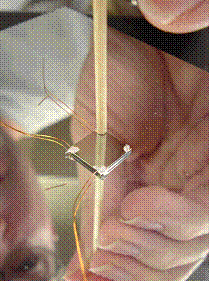
\includegraphics[width=0.4\linewidth]{images/SHEimage099.png}}
    \caption{Hughes Silvestri wires the Germanium sample, using Indium and a wooden rod.}
    \label{fig:SHEimage099}
\end{figure}

Once all the data have been collected, we are going to reverse the magnetic field and take the same data again. After that is done, we will turn off the magnetic field. (Actually, we will actively drive it to zero field with a small winding current. This overcomes residual hysteretic field.) We will take a third set of data at zero magnetic field (why?). \href{http://experimentationlab.berkeley.edu/hysteresis}{\textbf{What is hysteresis?}}

\section{Apparatus and Procedure}

In brief, this experiment involves measuring the resistivity and Hall voltage as functions of temperature on a particular semiconductor sample which has been prepared and mounted into a cryostat (Figure \ref{fig:OperatingPositionOfCryostat}). Components of the experiment you will be using are described below.

Temperature control system

To perform these measurements, we will first cool the sample to the lowest temperatures we will be accessing. This cooling of the apparatus is accomplished by adding liquid nitrogen to the cryostat twice: a first batch of liquid nitrogen will get the temperature down to about 240 K, and then we will keep adding nitrogen to lower the temperature further. A computer interfaced thermometric system is used to control the temperature. Once the specified lowest temperature is reached, a heater is turned on and the sample begins to slowly rise in temperature until the specified highest temperature is reached. This controlled temperature ramp can be terminated by stopping the experiment early. The computer will begin to record data every degree change as the temperature rises at 5K per minute. An upper temperature limit of 400 K is imposed so as not to damage the sample (in particular the leads on the sample. The sample we are going to use for this experiment is a doped germanium crystal that is cut out into an approximately 10mm x 10mm square +/- 0.01mm with thickness of approximately 1.25 millimeters +/- 0.01mm. The sample is mounted in a cryostat as shown in the Figure \ref{fig:OperatingPositionOfCryostat}. The germanium crystal is mounted to the front side of the copper block with connection leads A, B, C, and D. The backside of the copper block contains a silicon diode temperature sensor (DT-470/471/670 SD). This diode measures the temperature of the sample and is a two-lead device with a capability of a four-wire configuration for making more accurate measurements. The temperature range for the diode measurement is about 4K to 475K. Two wires out of four assigned to the diode are current leads, \emph{I±.} The diode's other two leads are for the voltage measurement, \emph{V±.} The copper block is mounted to the brass-copper rod containing a 50-watt maximum heating coil through which we will be able to heat up the sample. The brass part of the rod can be thought of as a thermal resistance: we want to limit how fast the sample cools and heats up. The whole assembly is submerged into the chamber in which part of it (copper block with the heating coil) lies in the vacuum and the other part in the chamber where liquid nitrogen will be poured (refer to Figure \ref{fig:OperatingPositionOfCryostat}). Vacuum is needed to keep the Germanium sample from oxidizing when it is heated above room temperature. The cryostat is kept between the poles of the magnet and serves to hold the magnetic field measurement probe in place perpendicular to the magnetic field.

\begin{figure}[h]
    \centering
    \href{http://experimentationlab.berkeley.edu/sites/default/files/images/SHEimage100.gif}{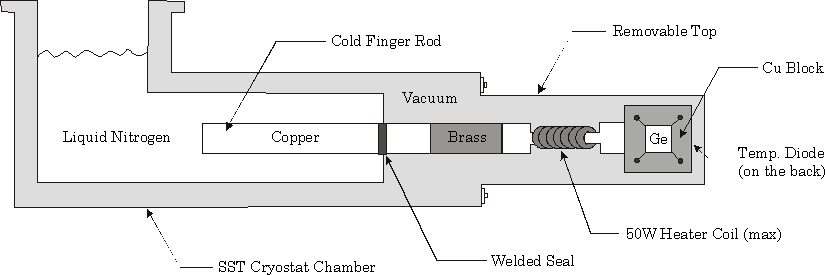
\includegraphics[width=0.7\linewidth]{images/SHEimage100.png}}
    \caption{Operating Position of the Cryostat}
    \label{fig:OperatingPositionOfCryostat}
\end{figure}

\begin{itemize}
    \item The two water valves are behind the magnet labelled ``Main Water'' (In) and ``Return'' (out). Open the Return 1st, then open SLOWLY the Main Water while pushing in and holding the button on the grey interlock box behind the magnet near the water valves. Check to see that you have 80 PSI water pressure on the meters on the table behind the magnet.
\end{itemize}

If NOT see \LabEngineer  immediately.

\begin{itemize}
    \item To turn off the water, close the Main Water(in) valve 1st, then monitor the water pressure on the meters and when it get to less then 5 PSI, turn off the Return valve.
\end{itemize}

In this experiment we are going to use 5000 Gauss electromagnet to observe the Hall effect. The electromagnet is powered by the two 60V DC power supplies connected in series. To prevent the magnet from overheating, water-cooling lines are connected to the magnet. Water interlock circuitry in the grey box monitors the flow of the water through the magnet. When it senses that there is no water circulation, this circuit prevents any significant operation of the magnet by tripping a disconnect relay whenever more than 5 watts are being dissipated into the magnet's coil. Magnet operation resumes as soon as water circulation is restored or the target field is reduced to close to zero. See Figure \ref{fig:SimpleBlockDiagram} for the simple block diagram of the experiment. Note that the data collection software still requires water to be flowing, at least at the beginning, even if measurements are being made at zero field.

The magnet is monitored by the LakeShore 450 Gaussmeter. It provides precise measurements of the magnetic fields. \emph{\textbf{To allow the LakeShore 450 to be used in a control loop to reach the target field, its auto-ranging and filtering have both been turned off (these settings persist even when turned off).}} To pass a current through any two leads of the sample we will use 2400 SourceMeter. To measure the voltage across any two leads of the sample we will use 6514 Electrometer. (These are finicky devices, sometimes needing to be turned off and back on again during the start of data-taking.) The 330 Temperature Controller measures and autonomously controls the temperature of the sample using the silicon diode temperature sensor. All these instruments are connected to the computer through a GPIB connection. The operation manuals of these instruments are contained in the Appendix B. {remember to TURN OFF the Temperature Controller when finish for the day, DO NOT LEAVE IT ON!!}

The Gold box is Labview computer controlled system that automatically triggers the 2400 Source meter to deliver its current to the sample. It also contains a bank of 16 relays to connect this current to one of four pairs of the sample's leads and measure the corresponding voltage on the remaining pair. The Labview program controls the Gold box and has the capability of switching the above, plus the magnetic field current and the sample current directions. It also monitors the status of the experiment and if something goes wrong, it has the capability to turn things off.


\begin{figure}[h]
    \centering
    \href{http://experimentationlab.berkeley.edu/sites/default/files/images/SHEimage101.gif}{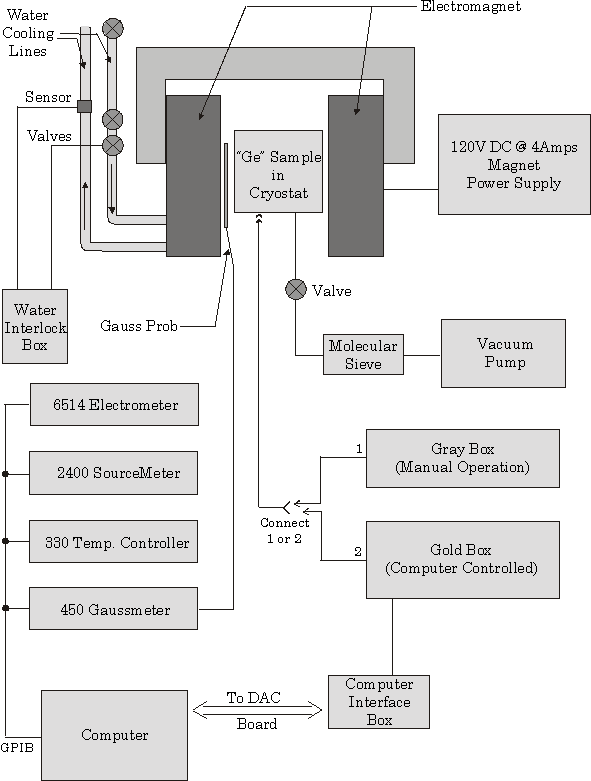
\includegraphics[width=0.7\linewidth]{images/SHEimage101.png}}
    \caption{Simple Block Diagram for the Hall Effect in Semiconductors experiment.}
    \label{fig:SimpleBlockDiagram}
\end{figure}

\section{Procedure}

Below is a ``simple'' procedure for this experiment.

Read the Cryogenic Safety sheet \textbf{before} filling the system with Liquid Nitrogen: See the Cryogenic Liquids information from EH\&S. \href{http://experimentationlab.berkeley.edu/sites/default/files/images/77cryogenic.pdf}{\textbf{Cryogenic Liquids}}

\textbf{Always wear the Blue Cryogenic safety gloves, the clear safety goggles, and the clear face shield while handling of LN-2.}

\subsection{Control Program procedure using the Gold box}

\begin{enumerate}
    \item Turn on the computer.

    \item Turn the water on. There are two valves that must be opened; first open the lever valve \textbf{Return} behind the magnet, then open the \textbf{Main Water} valve behind the magnet, and finally push the button on the grey interlock box. Hold the button for about 5 seconds. At first the light might blink but it should stop doing so in about a minute.

    \item Make sure the vacuum is below 100 milli-torr, plug in the pump and open the vacuum valve on the chamber. \textbf{NOTE: Keep Pump on during the time dewar is still cold, leave on overnight is okay.}

    \item Then turn on all the equipment in the Rack.

    \item Starting from the top most piece; Electrometer, Current Source, Gauss Meter, the Lakeshore Temperature Controller and the GOLD Box. The red on/off switch on the bottom of the top shelf indicated by a label ``POWER SWITCH" controls the power supply of all four devices in the rack. Then go to the two power supplies under the bench with the magnet on it and turn the power supplies on.

    \item Now push the ``RUN'' button on the GOLD Box (this button is located just above the on/off switch). The power supplies should turn on with a fan sound, if you turned on the circuit breakers on the power supplies.

    \item On your Desktop or in the Support folder on the C:$\backslash$ drive is the LabView Program called ``Control Program v9\_multifield'' execute this program, \href{http://experimentationlab.berkeley.edu/sites/default/files/images/SHE_FrontPanel.pdf}{\textbf{SHE Control Program Front Panel}}.

    \item The data that the program takes is as follows, \href{http://experimentationlab.berkeley.edu/sites/default/files/images/SHE_Data_Taking_Table.pdf}{\textbf{SHE Data Taking Table}}.

    \item Run the Control Program; Then input the experiment parameters; Sample Current, Magnet Field in Gauss ( Max 5000), Start Temperature, End Temperature (in K, Then click the Start Experiment button. Name a file to save with an extension of *.TXT or *.DAT for your data ( dialog Box will pop up).

    \item Test the system by inputting temperature range 120K to 200K.
    
    \checkpoint{Apparatus and Procedures}{Once you have taken your first testing run of system, explain the apparatus and the operating procedures to Professor or GSI.}

    \item Then you can use the defaults 95K to 350K the program will take about 1 hour 40 minutes to finish. The ``SAMPLE TEST CONDITION'' shown in the Figure \ref{fig:GoldBox.jpg} indicates the concurrent voltage and current measurement by two red and two green LEDs.

    \item You need to make 4 different sample current runs.

    \item Do NOT RUN or take data Overnight.

    \item \textbf{If you want to STOP early use the STOP button (Only Click it once) in the program DO NOT Stop LabView or X out the program. This would be like driving your car at 65 miles per hour and you get removed from your car while it is still going.} ( this takes about 60 seconds to stop)

    \item Wear the blue gloves and the face shield (available at your station) and with the help of a GSI fill the white dewar with liquid nitrogen. You do not actually need a full dewar.

    \item Now add some of the liquid nitrogen to the cryostat, so it can begin cooling. Move on to the next step, but periodically check the temperature displayed by the Lakeshore 330 Temperature Controller (check that it is on) and the Control Program display; when it reaches 240K, add more liquid nitrogen.(Always wear the blue gloves and a face shield while handling liquid nitrogen.) NOTE: You MUST add liquid nitrogen to the cryostat, even if you are only taking data for above room temperature.

    \item Check the temperature. The minimum temperature that we are capable of reaching is about 88K, but this is hard to get to; as long as you get bellow approximately 95K you should be fine. (88K takes about 1 hour to get)

    \item The Temperature Ramp Rate is set to increase the temperature by 2 Kelvin per minute (calculate how much time it will take for you to complete a run,  but remember, this is NOT an overnight lab: you must finish before closing time).

    \checkpoint{Extrapolating Data}{Once you have taken your first run of data determine what the Resistivity and Hall coefficients at room temperature are. How accurate are your measurements? What type of semiconductor are we dealing with (p-type or n-type) and how do you know this? At what temperature does the material transition between intrinsic and extrinsic? Finally, make sure you understand how to extrapolate the conductivity and find the ratio of the Hole and Electron Mobility at the point of transition between extrinsic and intrinsic regions (Talk to a GSI or review section 3.3 in Melissinos).}

    \item Run the procedure roughly 5 times and make sure you have enough data to analyze.

\end{enumerate}

\begin{enumerate}
    \item \textbf{When Finish for the day Stop Control Program or let it finish data taking.}

    \item \textbf{Turn off GOLD Box, and Heater controller before you leave the 111-Lab.}

\end{enumerate}

\subsection{Control Program Description}

\begin{enumerate}
    \item Start the Control Program ie; RUN LabView program

    \item Input Experiment Parameters

    \item Click Start Experiment

    \item The data taking will start after the start temperature is reached the second time.

    \item there is over shoot you will see it on the temperature graph.

    \item Temperature goes below set point then heater will come on and when start temperature is reached again data taking will start.

    \item NOTE: if for some reason the program crashes or you accidentally X out the program You must restart the program and just click start experiment button, with no parameters entered, to reset the system.

\end{enumerate}

Check to see that the Heater is OFF.

\begin{enumerate}
    \item \textbf{Turn off GOLD Box, and Heater controller when finished before you leave the 111-Lab.}

\end{enumerate}

\section{Report}

The following should be included in your report:

\begin{enumerate}
    \item Resistivity and Hall Coefficient of the sample at room temperature. At what magnetic field intensity, would the E field due to Hall effect be of the same magnitude (though perpendicular in direction) as the E field due to resistance?

    \item Plot of resistivity $\rho$ of the sample versus inverse temperature. Find at what temperature values the sample is in the extrinsic or intrinsic regions.

    \item Plot of conductivity $\sigma = 1/\rho$ versus inverse temperature.

    \item Plot of Hall coefficient of the sample versus inverse temperature.

    \item Calculate the carrier mobility ($\mu$) and carrier concentration (n).

    \item Plot (Hall coefficient X conductivity) versus $T$. Where does Hall coefficient becomes zero.

    \item Explain what type of material we have: p-type or n-type. (Why don't you need to know the direction of the magnetic field after all?)

    \item Find electron or hole concentrations for the sample versus temperature.\\
    \checkpoint{Electron or Hole Concentrations}{Explain to Professor or GSI which formulas you will use to find the electron or hole concentrations.}
    
    \item Find the Hall Coefficient $ R_H $ and the Hall mobility $\mu_H = R_H \cdot \sigma$ versus temperature.

    \item Find electron or hole concentration in the extrinsic region see \href{http://physics111.lib.berkeley.edu/Physics111/Reprints/SHE/24-Haller.pdf}{\textbf{E. Haller Article}}.

    \item Find electron \emph{and} hole mobilities in the extrinsic region.

    \item Compare the resistance measured for the sample (at zero field) with the magnetoresistance (the resistance measured while the magnetic field is on).

    \item Last day of the experiment please fill out the \href{\ExperimentEvaluation}{\textbf{Experiment Evaluation}}

\end{enumerate}

\section{References}
\label{sec:References}

\begin{enumerate}
    \item \href{http://experimentationlab.berkeley.edu/node/106}{\textbf{Instrument Manuals}}

    \item Neamen, D.A. ``\href{http://physics111.lib.berkeley.edu/Physics111/Reprints/SHE/09-Semiconductors.pdf}{\textbf{Ch.5: The Hall Effect pg. 17c, 180-183}}.'' \emph{Semiconductor Physics and Devices, Basic Principles} \href{http://physics111.lib.berkeley.edu/Physics111/Reprints/SHE/Donald_A._Neamen_Semiconductor_Physics_And_Devices_Basic_Principles.pdf}{\textbf{ (Whole Book)}}. (1992). More than you ever wanted to know about semiconductors.

    \item Preston and Dietz. ``\href{http://physics111.lib.berkeley.edu/Physics111/Reprints/SHE/07-Electrical\_Conductivity.pdf}{\textbf{Ch.17: Electrical Conductivity and the Hall Effect pg. 303-315}}.'' \emph{The Art of Experimental Physics} (1991).

    \item D. Halliday, R. Resnick, J. Walker. ``\href{http://physics111.lib.berkeley.edu/Physics111/Reprints/SHE/Halliday\_Resnick/Ch.\%2046\%20Conduction\%20of\%20electricity\%20in\%20solids.pdf}{\textbf{Chapter 46: Conduction of Electricity in Solids}} \emph{Fundamental of Physics extended.} Excellent introduction to conductivity in solids. (1993).

\end{enumerate}

\noindent Other reprints and reference materials can be found on the \href{http://physics111.lib.berkeley.edu/Physics111/Reprints/SHE/SHE\_index.html}{\textbf{Physics 111 Library Site}}

\end{document}
